% ============================================================================
% EV Charging Station Suitability Analysis — Project Report
% Compile with pdflatex or upload directly to Overleaf.com
% ============================================================================
\documentclass[12pt, a4paper]{article}

% ── Packages ────────────────────────────────────────────────────────────────
\usepackage[utf8]{inputenc}
\usepackage[T1]{fontenc}
\usepackage{lmodern}
\usepackage[margin=2.5cm]{geometry}
\usepackage{graphicx}
\usepackage{booktabs}
\usepackage{array}
\usepackage{longtable}
\usepackage{float}
\usepackage{amsmath}
\usepackage{hyperref}
\usepackage{xcolor}
\usepackage{listings}
\usepackage{caption}
\usepackage{subcaption}
\usepackage{enumitem}
\usepackage{fancyhdr}
\usepackage{titlesec}
\usepackage{cite}
\usepackage{url}
\usepackage{multirow}
\usepackage{tabularx}

% ── Hyperlink styling ──────────────────────────────────────────────────────
\hypersetup{
    colorlinks=true,
    linkcolor=blue!70!black,
    citecolor=blue!60!black,
    urlcolor=blue!80!black,
}

% ── Code listing styling ──────────────────────────────────────────────────
\lstset{
    basicstyle=\ttfamily\small,
    keywordstyle=\color{blue!80!black}\bfseries,
    commentstyle=\color{green!50!black}\itshape,
    stringstyle=\color{red!60!black},
    breaklines=true,
    frame=single,
    backgroundcolor=\color{gray!8},
    numbers=left,
    numberstyle=\tiny\color{gray},
    tabsize=4,
    showstringspaces=false,
}

% ── Header/Footer ─────────────────────────────────────────────────────────
\pagestyle{fancy}
\fancyhf{}
\fancyhead[L]{\small EV Charging Station Suitability Analysis}
\fancyhead[R]{\small \thepage}
\fancyfoot[C]{\small Banaras Hindu University}
\renewcommand{\headrulewidth}{0.4pt}
\renewcommand{\footrulewidth}{0.2pt}

% ── Title formatting ─────────────────────────────────────────────────────
\titleformat{\section}{\Large\bfseries}{\thesection.}{0.5em}{}
\titleformat{\subsection}{\large\bfseries}{\thesubsection.}{0.5em}{}
\titleformat{\subsubsection}{\normalsize\bfseries}{\thesubsubsection.}{0.5em}{}

% ============================================================================
%                            TITLE PAGE
% ============================================================================
\begin{document}

\begin{titlepage}
\centering
\vspace*{1.5cm}

{\Huge\bfseries EV Charging Station\\[0.3cm]
Suitability Analysis\\[0.5cm]}

{\Large\itshape Multispectral OSM Classification\\
\& Machine Learning--Based Site Prediction\\[1.5cm]}

\rule{\textwidth}{1.5pt}\\[0.5cm]

{\large
\textbf{A Project Report}\\[0.3cm]
Submitted in partial fulfilment of the requirements\\
for the course evaluation\\[1.5cm]
}

{\Large
\textbf{Submitted by:}\\[0.3cm]
\textit{Divyak -- 07}\\[0.3cm]
}

\vfill

{\large
\textbf{Department of Computer Science and Engineering}\\[0.2cm]
Indian Institute of Technology (BHU) / Banaras Hindu University\\
Varanasi -- 221005, India\\[0.5cm]
\textbf{April 2026}
}

\end{titlepage}

% ============================================================================
%                         TABLE OF CONTENTS
% ============================================================================
\newpage
\tableofcontents
\newpage

% ============================================================================
%                         1. INTRODUCTION
% ============================================================================
\section{Introduction}

\subsection{Background and Motivation}

India has witnessed a rapid surge in Electric Vehicle (EV) adoption, 
driven by government policies such as the FAME-II scheme, rising fuel 
prices, and growing environmental awareness. The Indian EV market is 
projected to reach 10 million annual sales by 2030 \cite{niti2022}. 
However, the growth of EVs is fundamentally constrained by the 
availability of charging infrastructure. Unlike conventional fuel 
stations, EV chargers must be strategically placed to minimise range 
anxiety, maximise utilisation, and ensure equitable access across 
urban and semi-urban spaces.

Current approaches to EV station placement in India are largely 
\textbf{ad hoc}---driven by land availability or commercial 
partnerships rather than data-driven spatial analysis. This leads to 
clustering of chargers in some areas while leaving vast regions 
underserved. University campuses, in particular, represent 
\textit{ideal testbeds} for EV charging infrastructure due to their 
well-defined boundaries, diverse building typologies (hostels, 
academic blocks, hospitals, sports complexes), multi-modal road 
networks, and high population density of early EV adopters (students 
and faculty).

\subsection{Problem Statement}

Given an arbitrary geographic area represented as an OpenStreetMap 
(OSM) file, the objectives are:

\begin{enumerate}[label=(\roman*)]
    \item \textbf{Classify} every spatial feature (roads, buildings, 
    land use, water bodies) into fine-grained categories using a 
    multispectral colour-coding scheme derived from OSM tags.
    \item \textbf{Score} each location for EV charging suitability 
    using a rule-based heuristic weighted model.
    \item \textbf{Train} a supervised Machine Learning classifier on 
    real-world EV charging station locations across Indian cities.
    \item \textbf{Predict} optimal EV charging station placement on 
    any new, unseen map using the trained ML model.
    \item \textbf{Visualise} results through 2D maps, 3D extruded 
    models, heatmaps, and ranked JSON reports.
\end{enumerate}

\subsection{Use Cases}

\begin{itemize}
    \item \textbf{Urban Planners:} Rapidly assess any area's readiness 
    for EV infrastructure using open data.
    \item \textbf{Municipal Bodies:} Prioritise budget allocation for 
    charger installation using data-backed rankings.
    \item \textbf{Campus Administrators:} Plan internal EV charging 
    networks for universities, tech parks, and hospitals.
    \item \textbf{Researchers:} Study spatial patterns of existing EV 
    infrastructure and their correlation with urban features.
    \item \textbf{EV Startups:} Identify high-demand, underserved 
    areas for new station deployment.
\end{itemize}

\subsection{Scope of the Project}

The prototype is built and demonstrated on three geographically 
diverse sites in India:

\begin{enumerate}
    \item \textbf{BHU Campus, Varanasi} — Primary study area 
    (1,300-acre campus with 15,162 OSM nodes, 1,686 ways).
    \item \textbf{IIT Delhi Campus, New Delhi} — Validation site 
    (compact urban campus).
    \item \textbf{Majestic Area, Bangalore} — Dense urban commercial 
    zone (high-density transit hub).
\end{enumerate}


% ============================================================================
%                       2. LITERATURE REVIEW
% ============================================================================
\section{Literature Review}

\subsection{EV Charging Station Placement}

Significant research exists on optimal EV charger placement using 
operations research and GIS-based methods. Key approaches include:

\begin{itemize}
    \item \textbf{Flow-based models:} The Flow-Refueling Location 
    Model (FRLM) optimises station placement along traffic corridors 
    to maximise intercepted vehicle flows.
    \item \textbf{GIS suitability analysis:} Multi-Criteria Decision 
    Analysis (MCDA) with weighted overlay of factors like road 
    proximity, land use, population density, and grid connectivity.
    \item \textbf{Machine Learning approaches:} Recent works apply 
    Random Forests, gradient boosting, and neural networks to predict 
    optimal locations from urban feature vectors.
\end{itemize}

\subsection{OpenStreetMap as a Data Source}

OpenStreetMap (OSM) is the world's largest crowdsourced geospatial 
database, containing over 10 billion data points. OSM data is 
available under the Open Database License (ODbL) and can be exported 
for any region in XML format (\texttt{.osm}). Key advantages include:

\begin{itemize}
    \item Free, open-access, globally available
    \item Rich tagging system for roads, buildings, amenities, and 
    land use
    \item Real-time queryable via the Overpass API
    \item Community-maintained and regularly updated
\end{itemize}

\subsection{Random Forest for Spatial Prediction}

Random Forest is an ensemble learning method that constructs multiple 
decision trees during training and outputs the class that is the mode 
of the individual trees. It is well-suited for spatial prediction 
because:

\begin{itemize}
    \item It handles mixed feature types (binary, count, continuous) 
    natively.
    \item It provides built-in feature importance via Mean Decrease 
    Impurity (MDI).
    \item It is robust to overfitting with proper hyperparameter 
    tuning.
    \item It does not require feature normalisation or scaling.
\end{itemize}


% ============================================================================
%                      3. SYSTEM ARCHITECTURE
% ============================================================================
\section{System Architecture}

The system is organised as a two-phase pipeline controlled by a 
unified entry point (\texttt{main.py}).

\subsection{High-Level Architecture}

\begin{figure}[H]
\centering
\fbox{\parbox{0.9\textwidth}{
\begin{verbatim}
  .osm file ──> Parse nodes & ways ──> Classify every feature
                                             |
              ┌──────────────────────────────┼──────────────────┐
              v                              v                  v
    2D Multispectral Map       EV Suitability Heatmap    3D Extruded Map
    (roads + buildings +       (scored + candidate        (buildings by
     land use)                  zone markers)              type + roads)
              |                              |                  |
              └──────────────────────────────┴──────────────────┘
                                             |
                              Legend Panel + JSON Report
                                             |
                              ┌──────────────┴──────────────┐
                              v                              v
                     ML Prediction Map              Feature Importance
                    (Random Forest prob.)              + CV AUC Plot
\end{verbatim}
}}
\caption{System architecture: two-phase pipeline.}
\label{fig:arch}
\end{figure}

\subsection{Project Structure}

\begin{table}[H]
\centering
\caption{Project files and their roles.}
\label{tab:project_structure}
\begin{tabular}{@{}ll@{}}
\toprule
\textbf{File} & \textbf{Role} \\
\midrule
\texttt{main.py} & Unified pipeline runner (CLI entry point) \\
\texttt{ev\_campus\_analyzer.py} & Phase 1: Multispectral OSM classification (928 LOC) \\
\texttt{ev\_ml\_predictor.py} & Phase 2: ML-based EV station prediction (888 LOC) \\
\texttt{identity.py} & Utility: inject EV station nodes into OSM files \\
\texttt{requirements.txt} & Python dependencies \\
\texttt{map.osm} & BHU campus OSM data (3.4~MB) \\
\texttt{ev-charging-stations-india.csv} & India-wide EV station dataset (228~KB) \\
\bottomrule
\end{tabular}
\end{table}

\subsection{Technology Stack}

\begin{table}[H]
\centering
\caption{Technology stack and dependencies.}
\label{tab:tech_stack}
\begin{tabular}{@{}lll@{}}
\toprule
\textbf{Component} & \textbf{Library} & \textbf{Purpose} \\
\midrule
Language & Python 3.8+ & Core implementation \\
XML Parsing & xml.etree.ElementTree & OSM file parsing \\
Numerical & NumPy & Array operations, Gaussian kernels \\
Visualisation & Matplotlib & 2D maps, 3D extrusion, heatmaps \\
ML Framework & scikit-learn & Random Forest, cross-validation \\
Data Handling & pandas & CSV I/O, feature matrix construction \\
Model Persistence & joblib & Save/load trained model \\
API Access & requests & Overpass API queries for training data \\
Fast XML (optional) & lxml & Accelerated parsing for large files \\
\bottomrule
\end{tabular}
\end{table}


% ============================================================================
%                    4. PHASE 1: MULTISPECTRAL CLASSIFICATION
% ============================================================================
\section{Phase 1: Multispectral OSM Classification}

\subsection{Overview}

Phase 1 ingests a raw \texttt{.osm} file and produces five output 
artefacts: a 2D classification map, an EV suitability heatmap, a 3D 
extruded map, a colour legend with statistics, and a JSON report. The  
entire phase operates offline and requires no internet access.

\subsection{OSM Parsing}

The \texttt{OSMParser} class reads the XML, extracting:
\begin{itemize}
    \item \textbf{Nodes:} Latitude, longitude, and optional tags for 
    each point.
    \item \textbf{Ways:} Ordered sequences of node references plus 
    key-value tags describing the feature.
    \item \textbf{Bounds:} The geographic bounding box 
    (\texttt{minlat}, \texttt{maxlat}, \texttt{minlon}, 
    \texttt{maxlon}).
\end{itemize}

For BHU: 15,162 nodes and 1,686 ways were parsed.

\subsection{Feature Classification}

The \texttt{classify\_way()} function is the classification engine. 
It inspects OSM tags in a priority order to assign each way to 
exactly one of \textbf{30+ categories}:

\subsubsection{Road Classification (by Hierarchy)}

Road width is not directly available in OSM for most ways. Instead, 
width is \emph{inferred} from the \texttt{highway=*} tag hierarchy:

\begin{table}[H]
\centering
\caption{Road classification by OSM highway type.}
\label{tab:roads}
\begin{tabular}{@{}llll@{}}
\toprule
\textbf{Colour} & \textbf{OSM Tag} & \textbf{Category} & \textbf{Approx.\ Width} \\
\midrule
Red-Orange & \texttt{primary} & Primary Road & $>12$~m \\
Amber & \texttt{secondary} & Secondary Road & 8--12~m \\
Yellow & \texttt{tertiary} & Tertiary Road & 6--8~m \\
Periwinkle & \texttt{residential} & Residential Road & $<6$~m \\
Light Grey & \texttt{service} & Service Road / Alley & narrow \\
Mint & \texttt{footway} & Footway / Pedestrian & --- \\
Turquoise & \texttt{cycleway} & Cycleway & --- \\
Tan & \texttt{path} / \texttt{track} & Unpaved Path & --- \\
\bottomrule
\end{tabular}
\end{table}

\subsubsection{Building Classification (by Function)}

Buildings are classified into 11 functional categories using a 
combination of:
\begin{itemize}
    \item Direct OSM tags: \texttt{building=*}, \texttt{amenity=*}, 
    \texttt{healthcare=*}, \texttt{leisure=*}, \texttt{tourism=*}
    \item \textbf{Name-based keyword matching}: Over 80 keywords 
    (e.g., ``hostel'', ``hospital'', ``canteen'', ``mandir'') are 
    matched against the \texttt{name=*} tag for buildings that lack 
    explicit functional tags.
\end{itemize}

Categories include: Academic/Lab, Hostel, Residential, Hospital, 
Temple, Sports, Library/Museum, Admin/Office, Canteen, Gate, and 
Generic (unclassified).

\subsubsection{Land Use and Natural Features}

Nine land-use categories are distinguished: Forest, Grassland, 
Garden/Park, Farmland, Barren/Open, Recreation, Water Body, Wetland, 
and Aquaculture.

\subsection{EV Suitability Scoring (Heuristic)}

Each OSM way is assigned a suitability score in $[0, 1]$ via a 
weighted additive model:

\begin{table}[H]
\centering
\caption{Heuristic EV suitability scoring weights.}
\label{tab:ev_score}
\begin{tabular}{@{}lr@{}}
\toprule
\textbf{Criterion} & \textbf{Weight} \\
\midrule
Primary / secondary road access & $+0.40$ \\
Parking area & $+0.35$ \\
University / college amenity & $+0.30$ \\
Hospital / library nearby & $+0.25$ \\
Conference / community centre & $+0.22$ \\
Education land use & $+0.20$ \\
Name keywords (gate, parking, main entry) & $+0.20$ \\
Restaurant / cafe (footfall proxy) & $+0.12$ \\
Recreation ground & $+0.12$ \\
Water body / waterway (penalty) & $-0.20$ to $-0.30$ \\
\bottomrule
\end{tabular}
\end{table}

The scoring function is used in two ways:
\begin{enumerate}
    \item To generate the \textbf{suitability heatmap} (output 02) via 
    Gaussian kernel density estimation on a $250 \times 250$ grid.
    \item To produce the \textbf{ranked candidate zone list} in the 
    JSON report (output 05).
\end{enumerate}

\textbf{Priority tiers:}
\begin{itemize}
    \item \textcolor{green!70!black}{\textbf{HIGH}} ($\geq 0.55$): 
    Strong candidate zone
    \item \textcolor{orange!80!black}{\textbf{MEDIUM}} ($0.40$--$0.54$): 
    Moderate candidate
    \item \textcolor{red!70!black}{\textbf{LOW}} ($< 0.40$): Lower 
    priority
\end{itemize}

\subsection{3D Visualisation}

Buildings are extruded to pseudo-3D heights based on their functional 
category:

\begin{table}[H]
\centering
\caption{Default extrusion heights by building category.}
\label{tab:3d_heights}
\begin{tabular}{@{}lr@{}}
\toprule
\textbf{Category} & \textbf{Relative Height} \\
\midrule
Academic / Dept / Lab & 0.060 \\
Hospital / Medical & 0.050 \\
Temple / Place of Worship & 0.045 \\
Library / Museum & 0.042 \\
Hostel / Student Housing & 0.040 \\
Admin / Office & 0.038 \\
Sports / Pool & 0.035 \\
Residential (Staff) & 0.030 \\
Canteen / Cafe & 0.025 \\
Generic (Unclassified) & 0.020 \\
Gate / Entrance & 0.015 \\
\bottomrule
\end{tabular}
\end{table}

When the OSM \texttt{height=*} tag is present, the actual height is 
used (capped at 0.12 relative units for visual clarity). Land-use 
patches are rendered as flat ground layers at near-zero elevations.

\subsection{Phase 1 Outputs}

\begin{figure}[H]
\centering
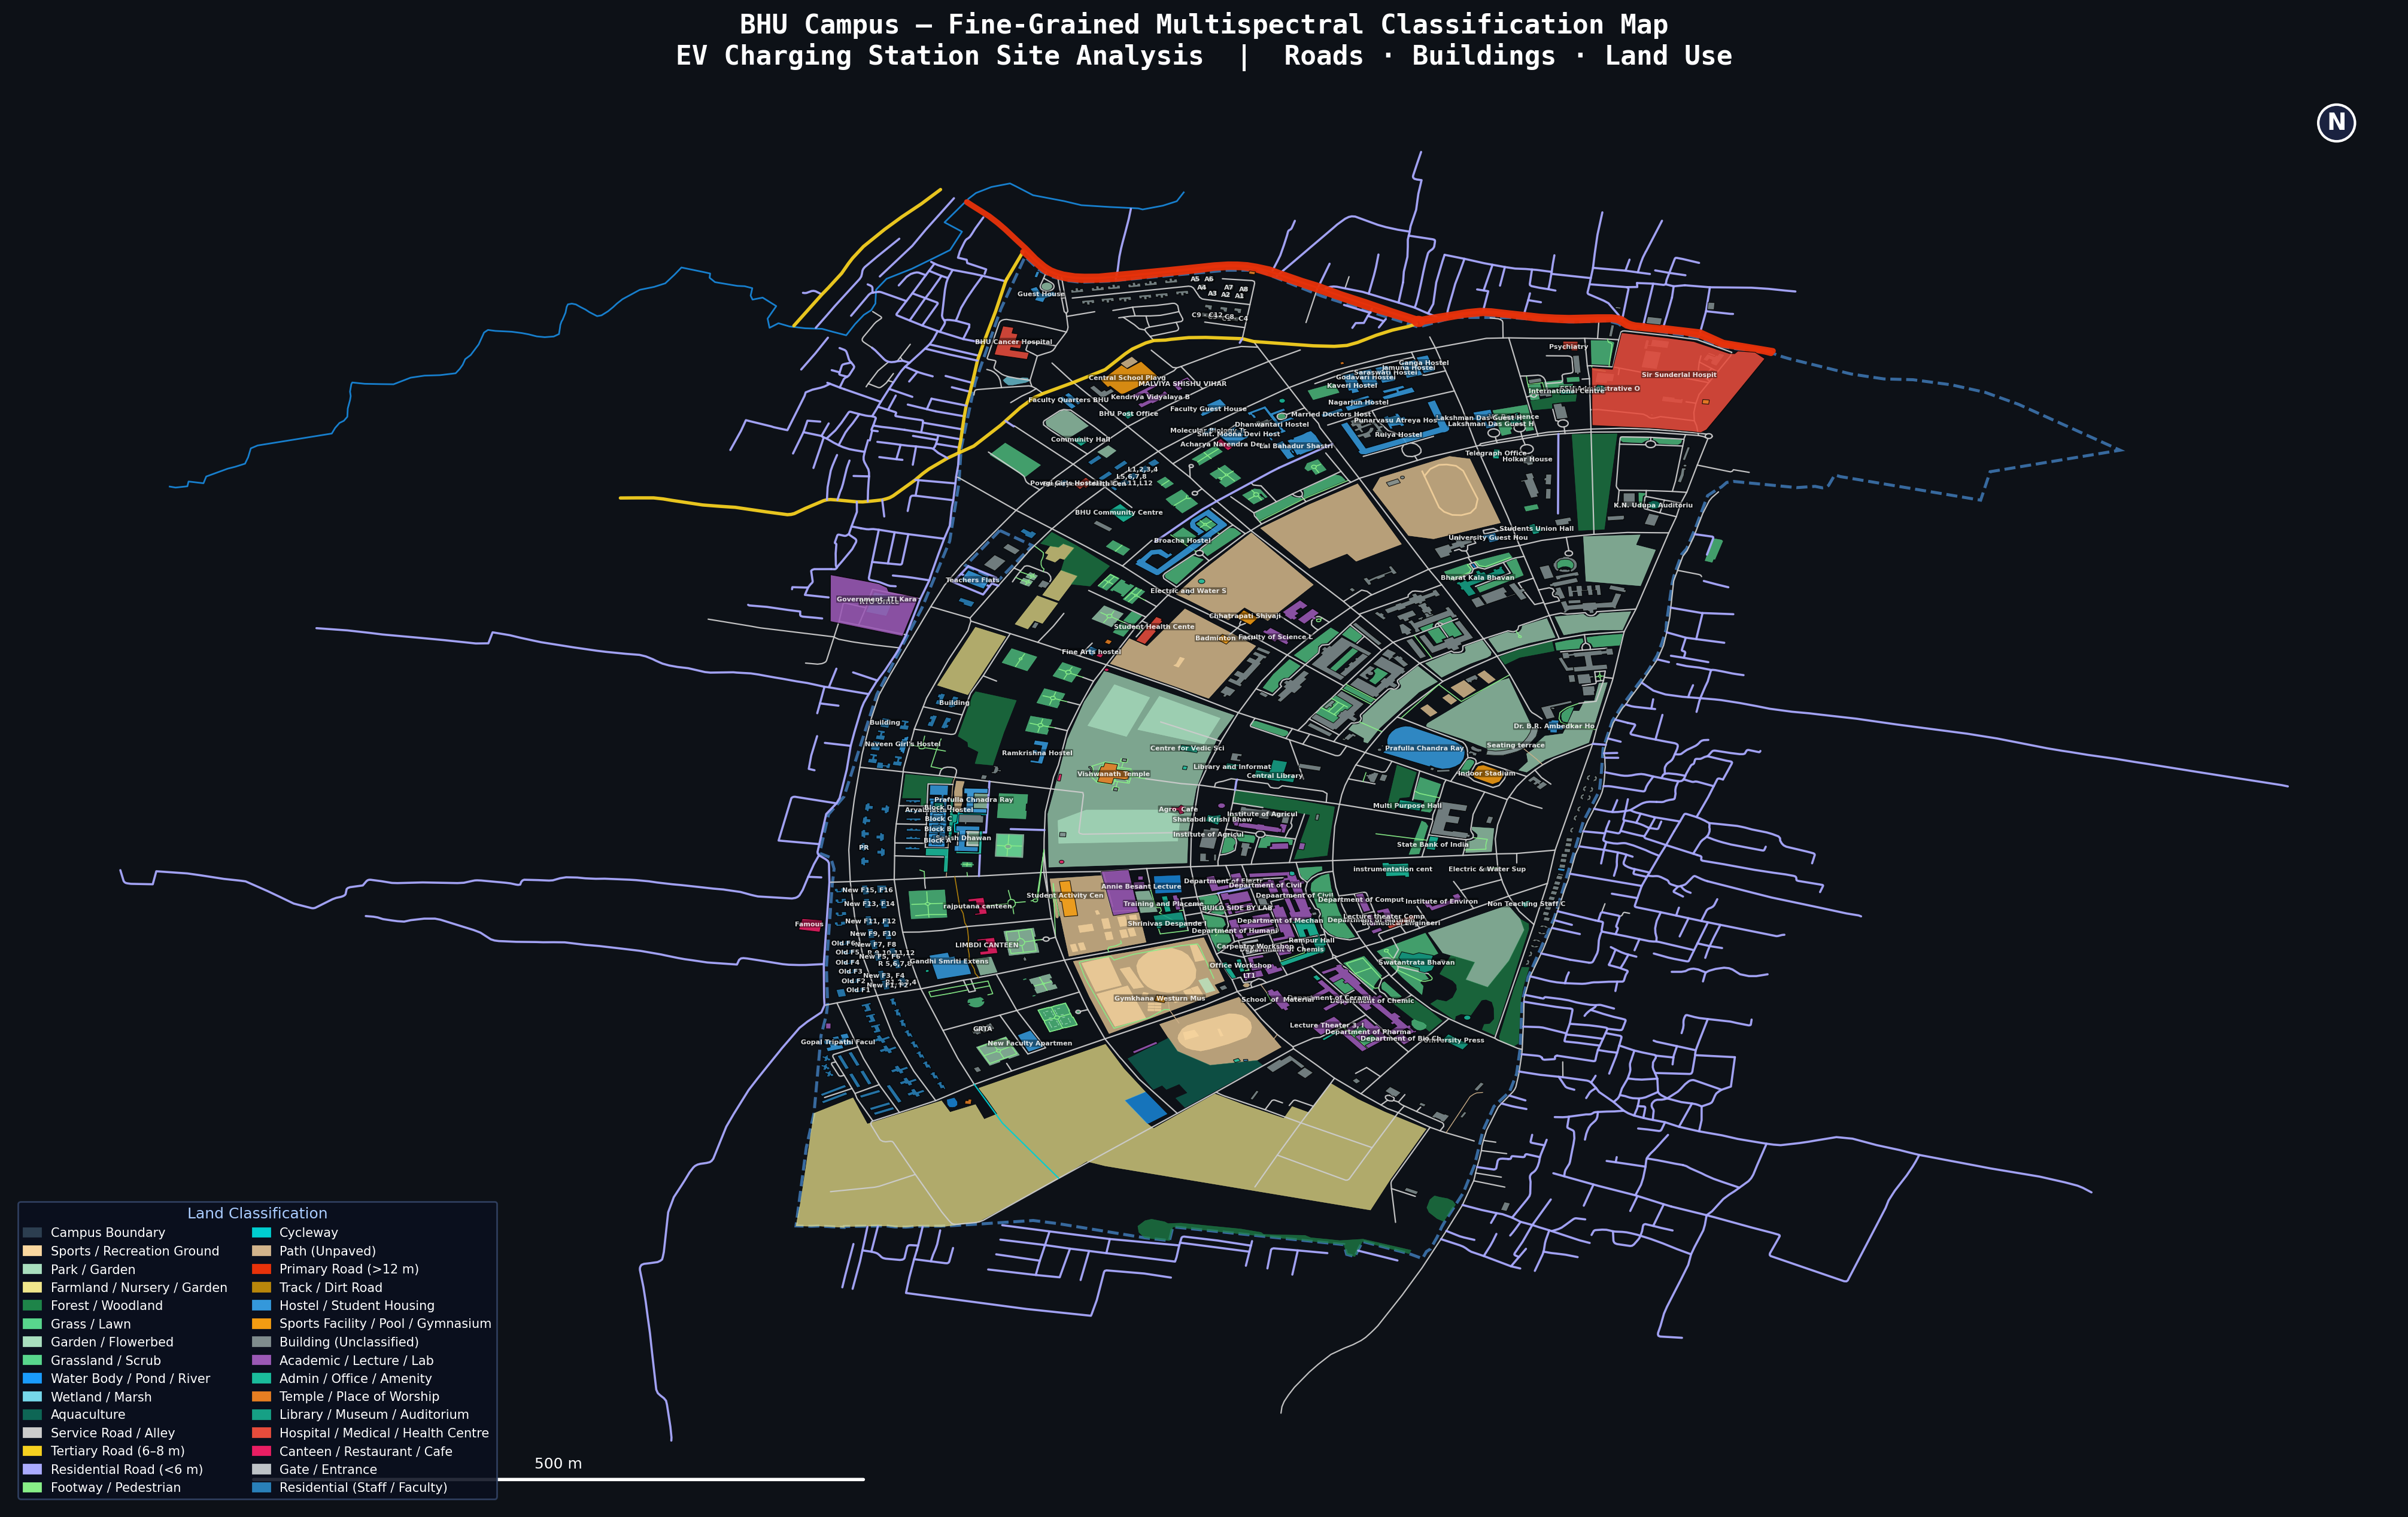
\includegraphics[width=0.95\textwidth]{figures/bhu_multispectral.png}
\caption{2D Multispectral Classification Map for BHU Campus. Each 
feature is colour-coded by its functional category: roads by 
hierarchy, buildings by function, and land patches by type. The 
dashed blue outline shows the campus boundary.}
\label{fig:bhu_multispectral}
\end{figure}

\begin{figure}[H]
\centering
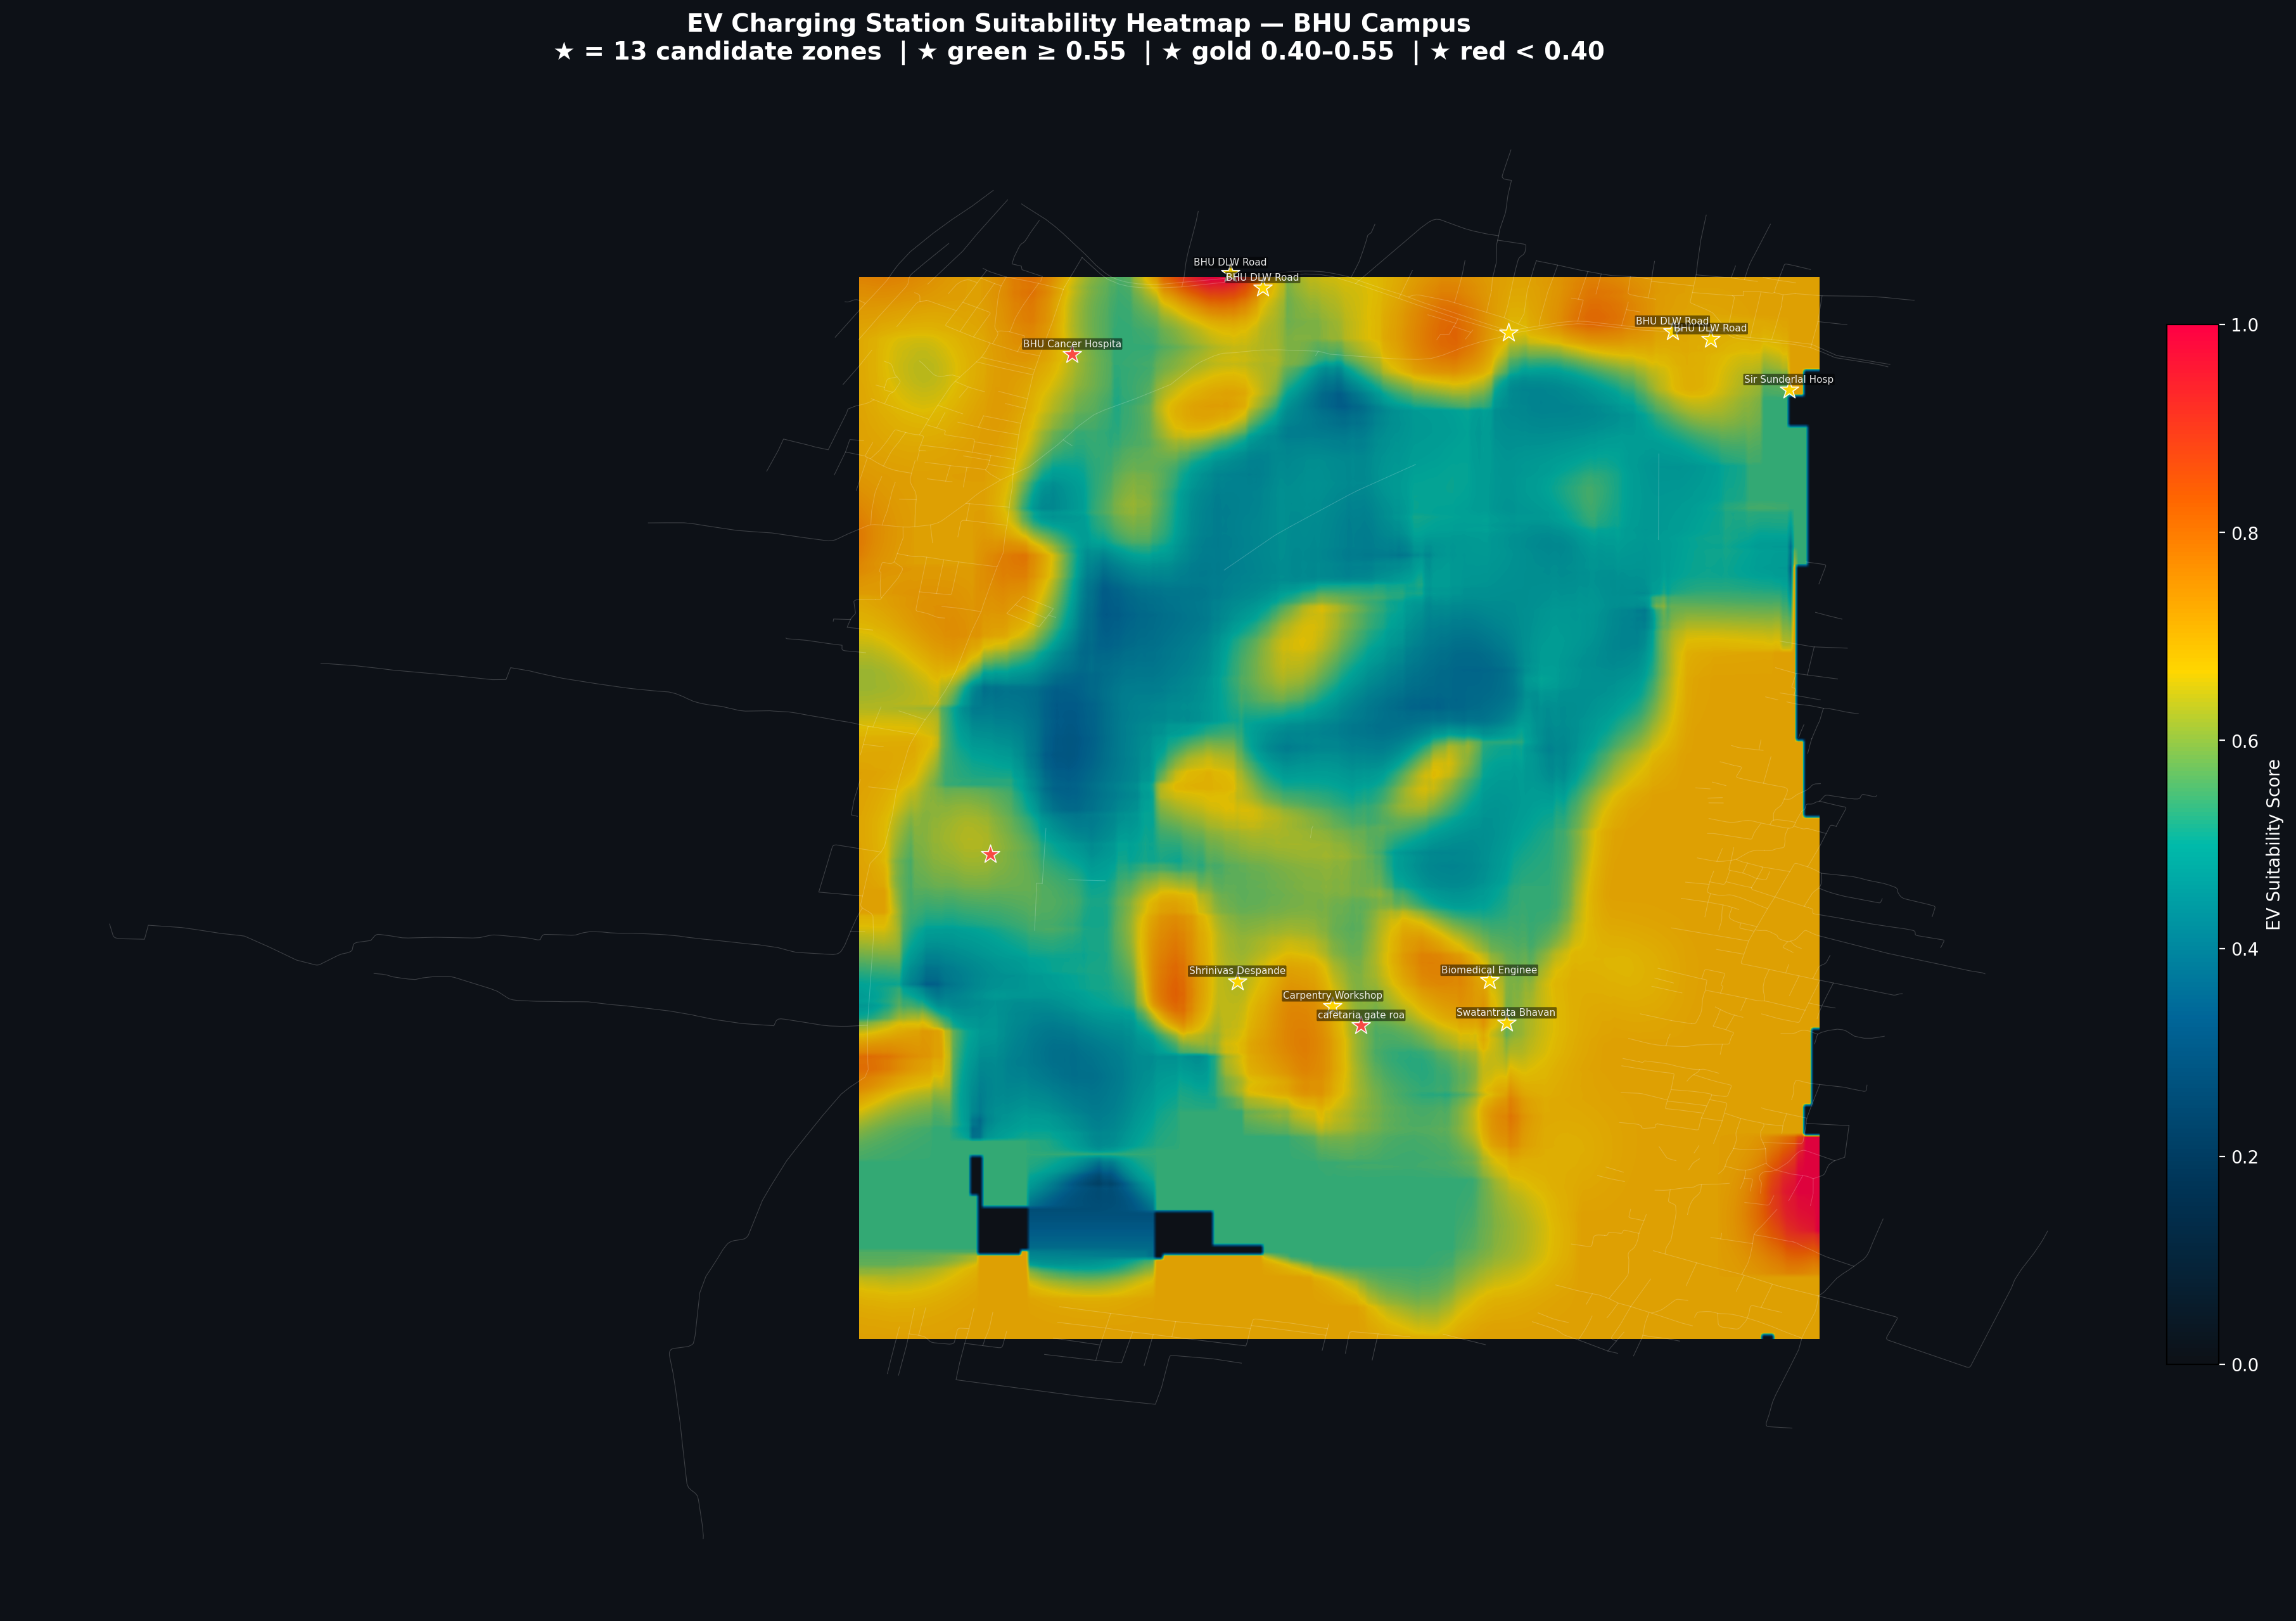
\includegraphics[width=0.90\textwidth]{figures/bhu_heatmap.png}
\caption{EV Suitability Heatmap for BHU Campus. Star markers 
indicate the top candidate zones. The colour scale ranges from cool 
(low suitability) to warm (high suitability) based on the weighted 
scoring model.}
\label{fig:bhu_heatmap}
\end{figure}

\begin{figure}[H]
\centering
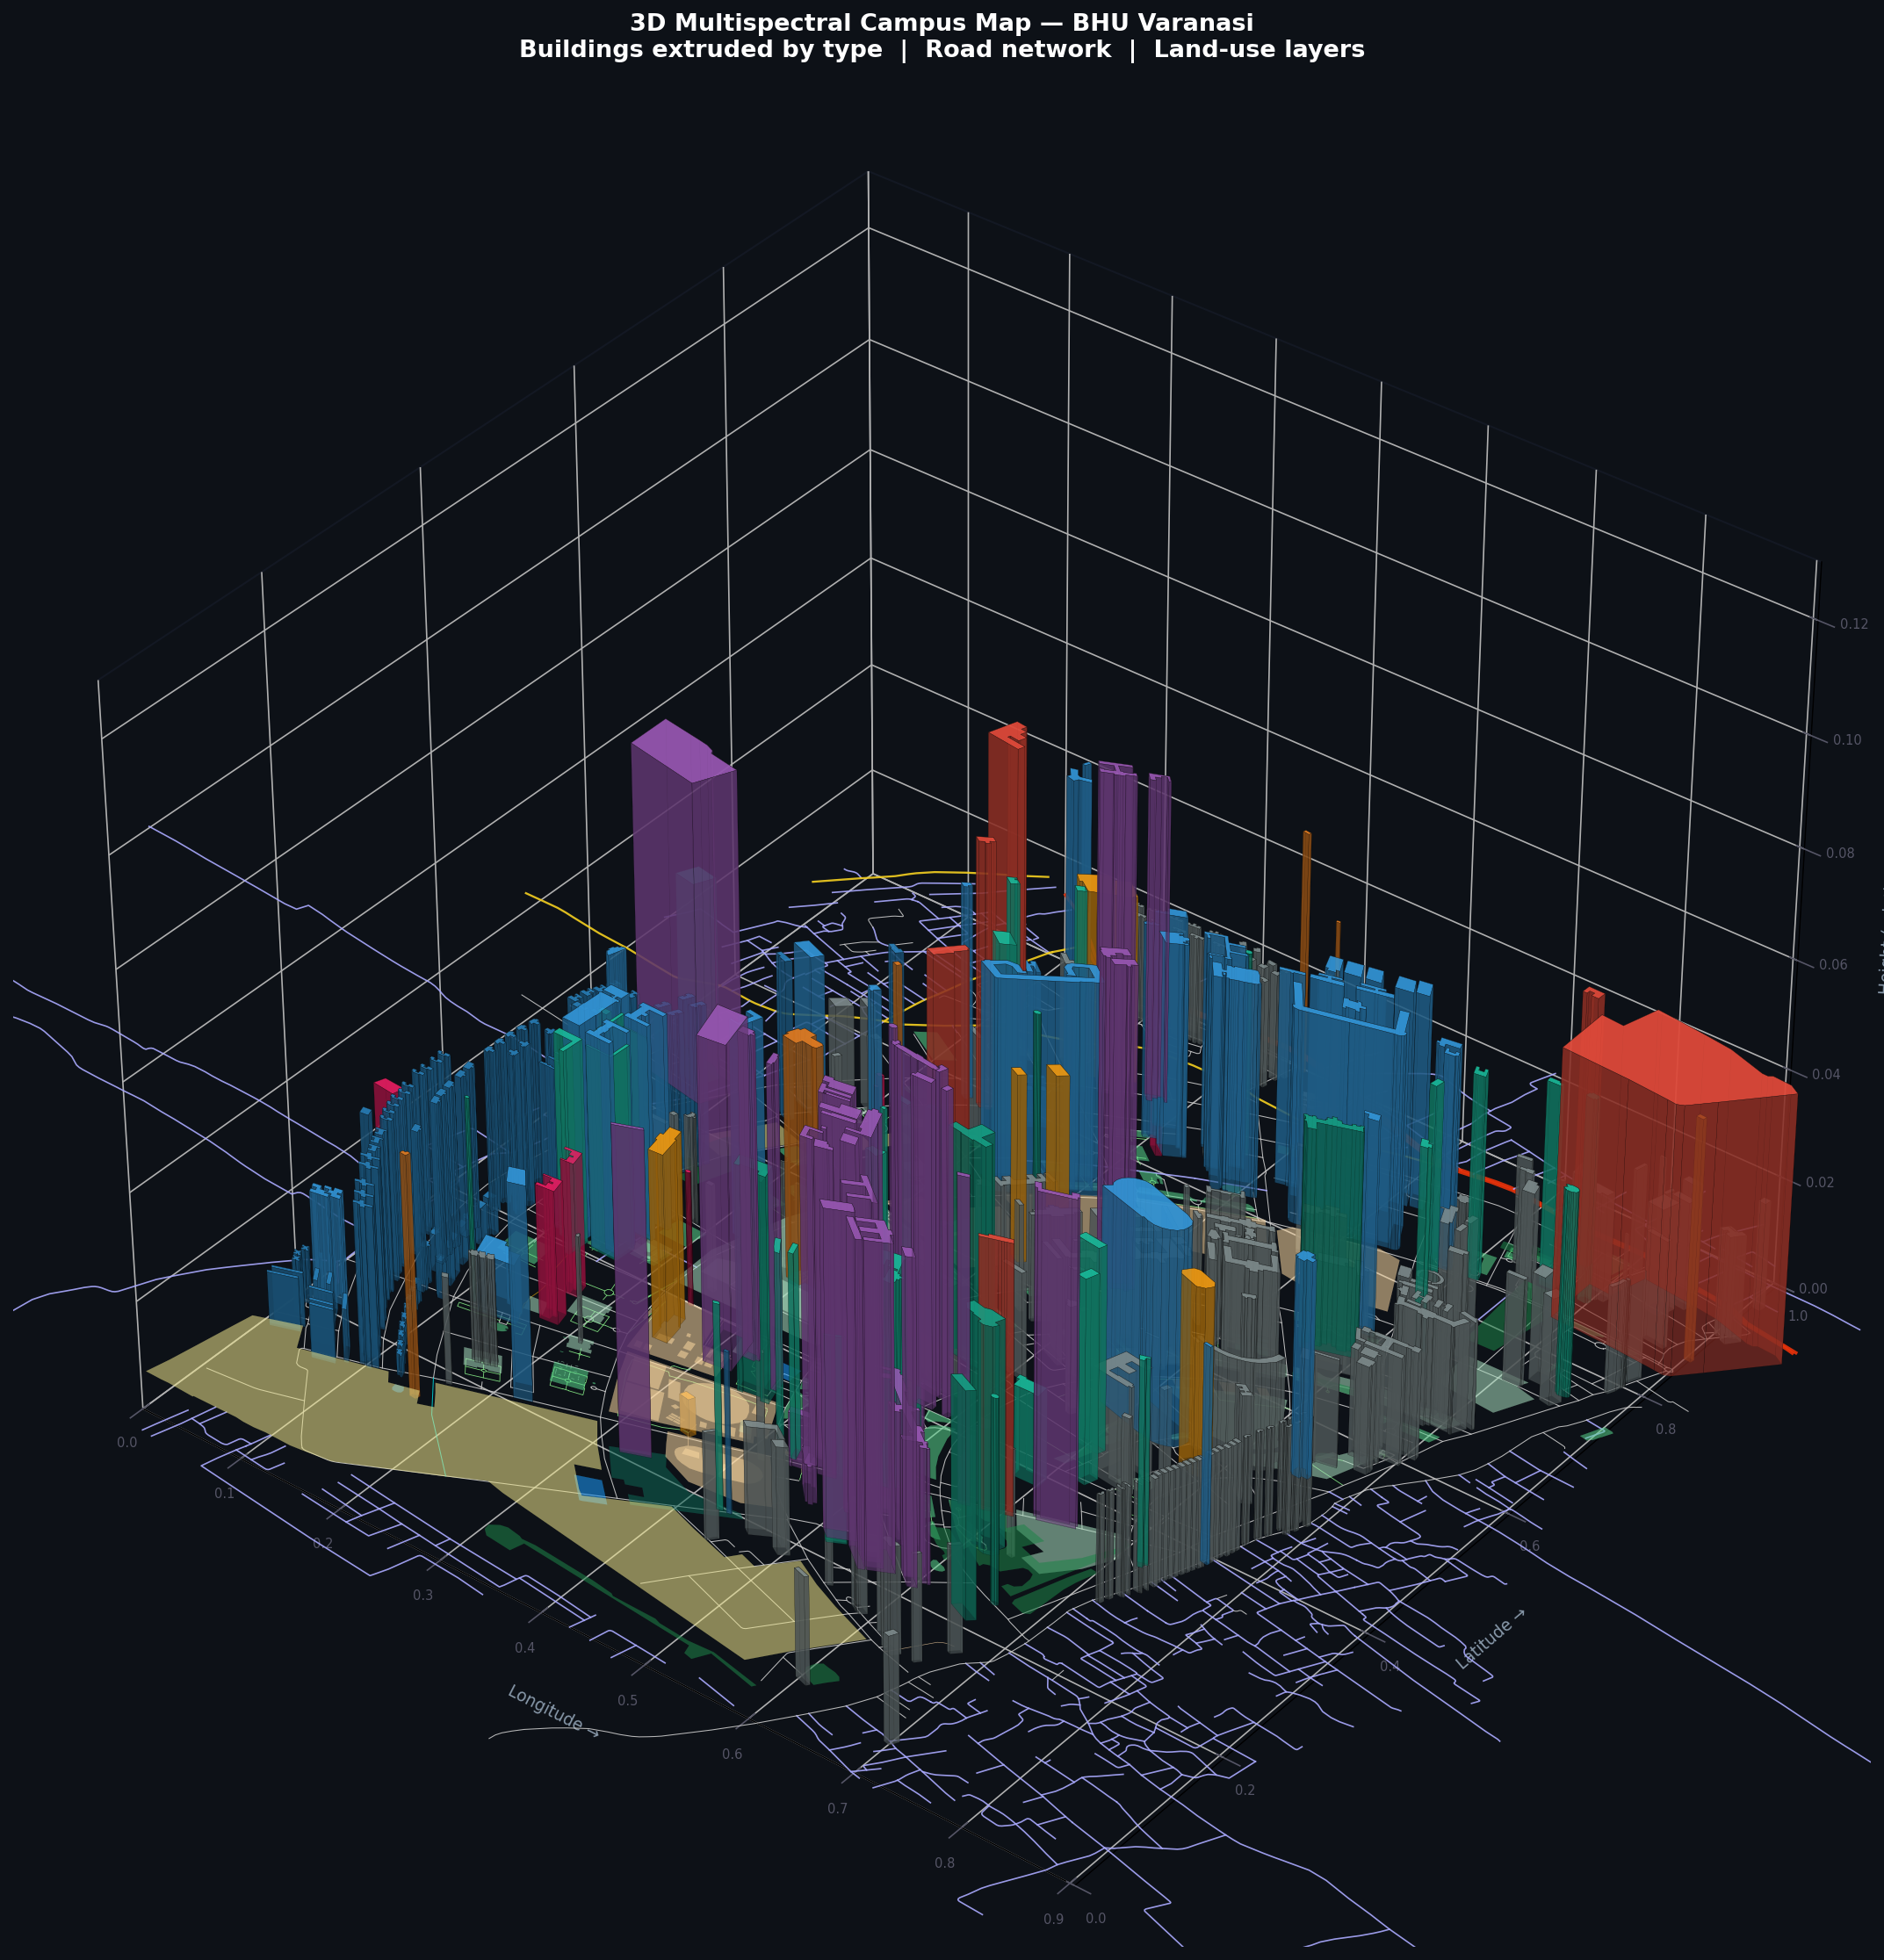
\includegraphics[width=0.85\textwidth]{figures/bhu_3d.png}
\caption{3D Extruded Multispectral Map of BHU Campus. Buildings are 
extruded based on their functional category. Academic blocks (violet) 
are tallest; generic buildings (grey) are shortest. Land-use layers 
and roads are rendered on the ground plane.}
\label{fig:bhu_3d}
\end{figure}


% ============================================================================
%                 5. PHASE 2: ML-BASED PREDICTION
% ============================================================================
\section{Phase 2: Machine Learning--Based EV Station Prediction}

\subsection{Motivation for ML}

While the heuristic scoring in Phase 1 provides reasonable results 
within a single map, it has inherent limitations:

\begin{itemize}
    \item Feature weights are manually assigned, introducing subjective 
    bias.
    \item It cannot learn from real-world patterns of where EV 
    stations are actually built.
    \item It does not generalise---each new criterion requires manual 
    coding.
\end{itemize}

Phase 2 addresses this by training a supervised ML model on 
\textbf{real, existing EV charging station locations} across Indian 
cities, learning the spatial feature patterns that characterise 
successful station placements, and applying those learned patterns 
to predict suitability on any new, unseen map.

\subsection{Training Data Generation}

\subsubsection{Data Source}

The training data source is \texttt{ev-charging-stations-india.csv} 
(228~KB), a dataset containing latitude/longitude coordinates of 
existing EV charging stations across India.

\subsubsection{Feature Extraction via Overpass API}

For each station, the pipeline:

\begin{enumerate}
    \item Queries the free \textbf{Overpass API} for all OSM elements 
    (nodes, ways, relations) within a 500-metre radius of the 
    station's coordinates.
    \item Extracts \textbf{23 spatial features} from the returned 
    elements (described in Section~\ref{sec:features}).
    \item Labels the sample as \textbf{positive} (label = 1).
    \item Generates $k = 2$ \textbf{negative samples} by offsetting 
    the coordinates by $\sim$1.5~km in random directions (areas 
    unlikely to host a charging station) and querying their features.
    \item Introduces a \textbf{2-second delay} between API calls 
    to respect rate limits.
\end{enumerate}

Up to 150 stations are sampled across multiple cities for diversity. 
The generated training data is cached to 
\texttt{output/training\_data.csv} (433 samples in our run) for 
reproducibility and fast iteration.

\subsection{Feature Engineering}
\label{sec:features}

Each sample (both positive and negative) is represented by a 
23-dimensional feature vector:

\begin{table}[H]
\centering
\caption{Complete feature vector (23 features).}
\label{tab:features}
\small
\begin{tabular}{@{}rll@{}}
\toprule
\textbf{\#} & \textbf{Feature Name} & \textbf{Description} \\
\midrule
1 & \texttt{road\_primary} & Binary: primary road within radius \\
2 & \texttt{road\_secondary} & Binary: secondary road within radius \\
3 & \texttt{road\_tertiary} & Binary: tertiary road within radius \\
4 & \texttt{road\_residential} & Binary: residential road within radius \\
5 & \texttt{road\_service} & Binary: service road within radius \\
6 & \texttt{road\_any} & Binary: any road within radius \\
7 & \texttt{road\_count\_norm} & Normalised count of road segments \\
8 & \texttt{parking\_nearby} & Binary: parking amenity detected \\
9 & \texttt{amenity\_university} & Binary: university/college nearby \\
10 & \texttt{amenity\_hospital} & Binary: hospital/clinic nearby \\
11 & \texttt{amenity\_restaurant\_cafe} & Binary: restaurant/cafe nearby \\
12 & \texttt{amenity\_bank} & Binary: bank/ATM nearby \\
13 & \texttt{amenity\_school} & Binary: school nearby \\
14 & \texttt{amenity\_conference} & Binary: conference centre nearby \\
15 & \texttt{amenity\_any} & Normalised count of any amenities \\
16 & \texttt{landuse\_education} & Binary: education land use \\
17 & \texttt{landuse\_commercial} & Binary: commercial land use \\
18 & \texttt{landuse\_residential} & Binary: residential land use \\
19 & \texttt{landuse\_recreation} & Binary: recreation land use \\
20 & \texttt{building\_count\_norm} & Normalised building count \\
21 & \texttt{node\_density} & Normalised total OSM node count \\
22 & \texttt{has\_existing\_ev} & Binary: existing EV station tag \\
23 & \texttt{poi\_density} & Normalised POI (shop, tourism, etc.) count \\
\bottomrule
\end{tabular}
\end{table}

\subsection{Model Architecture}

A \textbf{Random Forest Classifier} is used with the following 
hyperparameters:

\begin{table}[H]
\centering
\caption{Random Forest hyperparameters.}
\label{tab:rf_params}
\begin{tabular}{@{}ll@{}}
\toprule
\textbf{Parameter} & \textbf{Value} \\
\midrule
Number of trees (\texttt{n\_estimators}) & 300 \\
Maximum depth (\texttt{max\_depth}) & 10 \\
Class weight balancing & \texttt{balanced} \\
Random state & 42 \\
Bootstrap sampling & True (default) \\
Split criterion & Gini impurity \\
\bottomrule
\end{tabular}
\end{table}

The \texttt{class\_weight='balanced'} option automatically adjusts 
weights inversely proportional to class frequencies, addressing the 
class imbalance inherent in sampling (2 negatives per 1 positive).

\subsection{Training and Validation}

\subsubsection{Cross-Validation Strategy}

The model is evaluated using \textbf{5-fold Stratified 
Cross-Validation} with \textbf{ROC-AUC} as the scoring metric, 
ensuring that class proportions are maintained across all folds.

\begin{figure}[H]
\centering
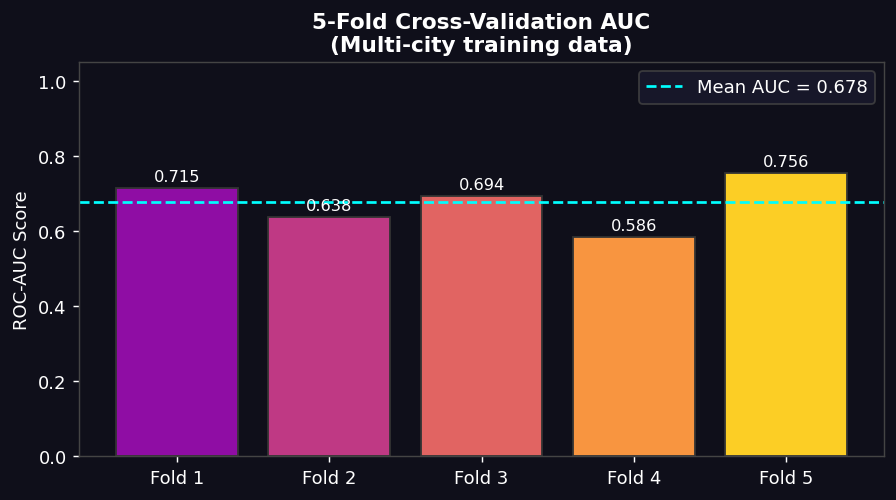
\includegraphics[width=0.55\textwidth]{figures/cv_auc.png}
\caption{5-fold stratified cross-validation ROC-AUC scores. 
Mean AUC = 0.678 across all folds.}
\label{fig:cv_auc}
\end{figure}

\begin{table}[H]
\centering
\caption{Cross-validation results per fold.}
\label{tab:cv_results}
\begin{tabular}{@{}lr@{}}
\toprule
\textbf{Fold} & \textbf{ROC-AUC} \\
\midrule
Fold 1 & 0.715 \\
Fold 2 & 0.638 \\
Fold 3 & 0.694 \\
Fold 4 & 0.586 \\
Fold 5 & 0.756 \\
\midrule
\textbf{Mean} & \textbf{0.678} \\
\bottomrule
\end{tabular}
\end{table}

A mean AUC of 0.678 indicates that the model performs meaningfully 
above random chance (0.5) at distinguishing suitable from unsuitable 
locations, though there is room for improvement with richer training 
data and additional features.

\subsubsection{Feature Importance}

\begin{figure}[H]
\centering
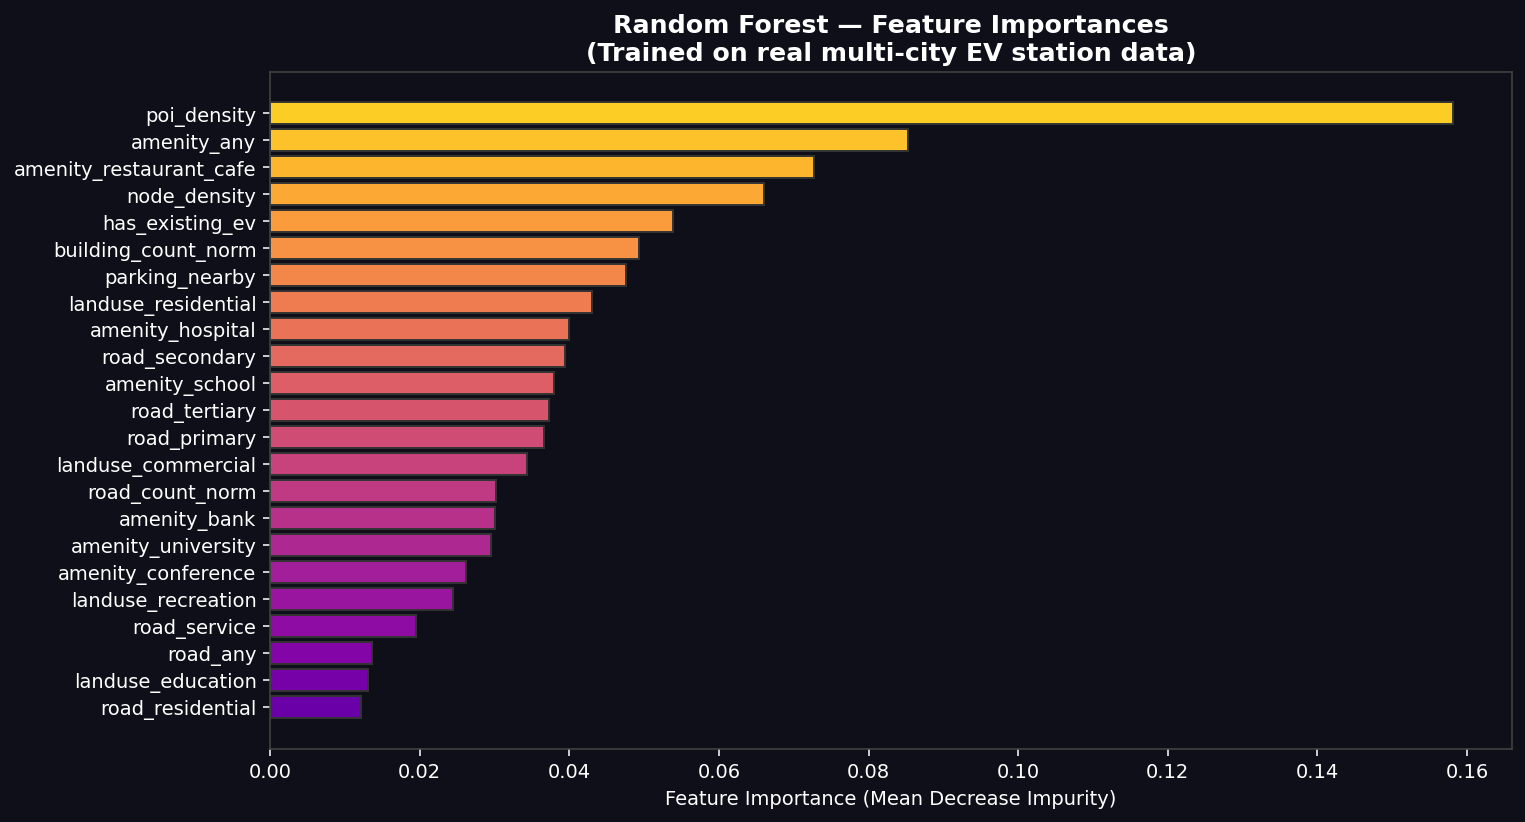
\includegraphics[width=0.82\textwidth]{figures/feature_importance.png}
\caption{Random Forest feature importances ranked by Mean Decrease 
Impurity (MDI). POI density, overall amenity count, and 
restaurant/cafe presence are the most discriminative features.}
\label{fig:feature_importance}
\end{figure}

Key findings from the feature importance analysis:
\begin{enumerate}
    \item \textbf{\texttt{poi\_density}} (0.16) — the single most 
    important feature; real EV stations are located in areas with 
    high Point-of-Interest density.
    \item \textbf{\texttt{amenity\_any}} (0.09) — general amenity 
    count strongly distinguishes positive from negative samples.
    \item \textbf{\texttt{amenity\_restaurant\_cafe}} (0.07) — 
    restaurants and cafes serve as proxies for foot traffic and dwell 
    time.
    \item \textbf{\texttt{node\_density}} (0.07) — raw OSM data 
    density correlates with urban development intensity.
    \item \textbf{\texttt{has\_existing\_ev}} (0.06) — co-location 
    of multiple chargers in the same zone is a strong signal.
\end{enumerate}

\subsection{Prediction Pipeline}

Once the model is trained and saved as \texttt{ev\_model.joblib}, 
prediction on a new map proceeds as follows:

\begin{enumerate}
    \item Parse the \texttt{.osm} file to extract all nodes, ways, 
    and the bounding box.
    \item Build a \textbf{spatial index} for efficient neighbour 
    lookups.
    \item Divide the bounding box into a \textbf{grid} with 
    $\sim$111-metre cell resolution.
    \item For each grid cell, extract the 23-feature vector by 
    querying the spatial index for elements within a 
    $\sim$330-metre radius.
    \item Feed the feature matrix to the trained Random Forest and 
    obtain \textbf{class probabilities} $P(\text{suitable})$ for 
    each cell.
    \item Deduplicate and rank the top candidates.
    \item Generate output maps and JSON report.
\end{enumerate}

This prediction step is \textbf{entirely offline} and completes in 
under 10 seconds for typical campus-sized maps.

\subsection{Phase 2 Outputs}

\begin{figure}[H]
\centering
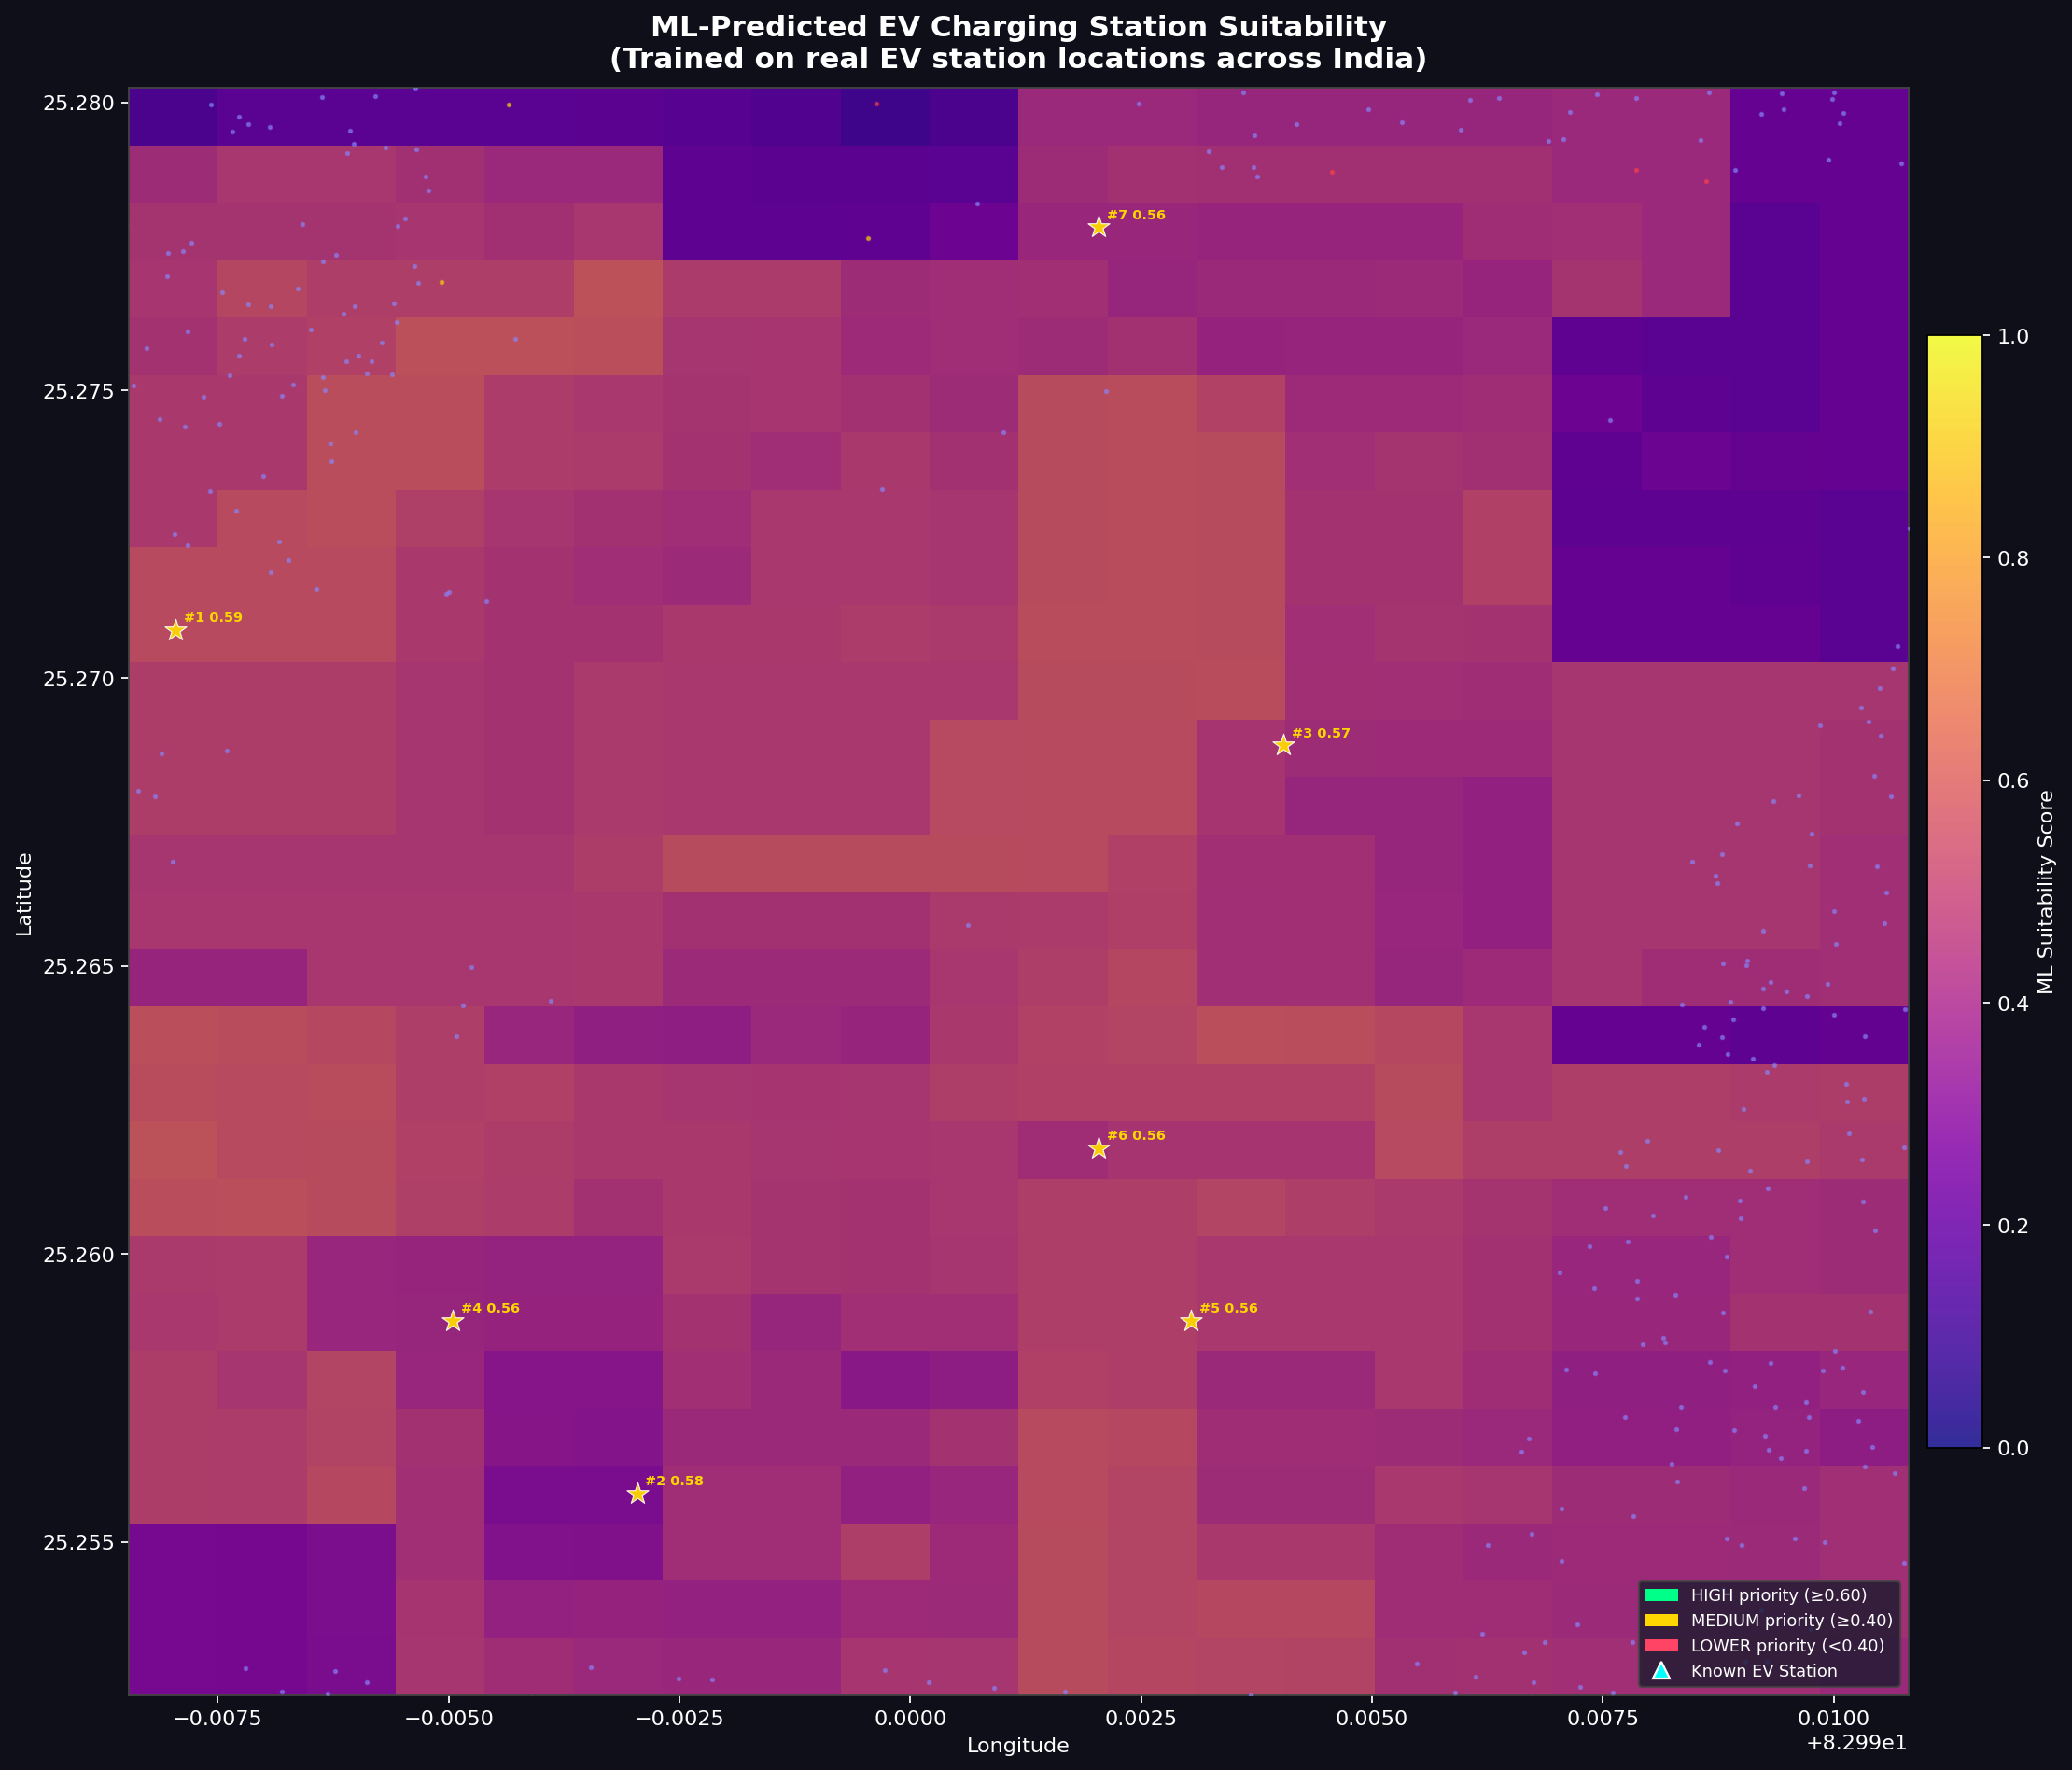
\includegraphics[width=0.80\textwidth]{figures/bhu_ml_prediction.png}
\caption{ML-Predicted EV Charging Station Suitability for BHU 
Campus. Star markers show the top-ranked candidate zones with their 
ML scores. The colour scale represents predicted probability of 
suitability (0 to 1).}
\label{fig:bhu_ml_prediction}
\end{figure}


% ============================================================================
%                         6. RESULTS
% ============================================================================
\section{Results and Case Studies}

\subsection{Case Study 1: BHU Campus, Varanasi}

\begin{table}[H]
\centering
\caption{BHU Campus — heuristic top EV candidate zones (Phase 1).}
\label{tab:bhu_heuristic}
\begin{tabular}{@{}rlccl@{}}
\toprule
\textbf{Rank} & \textbf{Location Name} & \textbf{Lat} & \textbf{Lon} & \textbf{Score / Priority} \\
\midrule
1 & Swatantrata Bhavan & 25.2606 & 82.9945 & 0.47 / MEDIUM \\
2 & Carpentry Workshop & 25.2611 & 82.9910 & 0.45 / MEDIUM \\
3 & Main Library (IIT-BHU) & 25.2617 & 82.9891 & 0.45 / MEDIUM \\
4 & Sir Sunderlal Hospital & 25.2773 & 83.0002 & 0.40 / MEDIUM \\
5 & BHU DLW Road & 25.2786 & 82.9986 & 0.40 / MEDIUM \\
\bottomrule
\end{tabular}
\end{table}

\begin{table}[H]
\centering
\caption{BHU Campus — ML-predicted top EV candidate zones (Phase 2).}
\label{tab:bhu_ml}
\begin{tabular}{@{}rccl@{}}
\toprule
\textbf{Rank} & \textbf{Latitude} & \textbf{Longitude} & \textbf{ML Score / Tier} \\
\midrule
1 & 25.27084 & 82.98204 & 0.5856 / MEDIUM \\
2 & 25.25584 & 82.98704 & 0.5785 / MEDIUM \\
3 & 25.26884 & 82.99404 & 0.5690 / MEDIUM \\
4 & 25.25884 & 82.98504 & 0.5637 / MEDIUM \\
5 & 25.25884 & 82.99304 & 0.5612 / MEDIUM \\
6 & 25.26184 & 82.99204 & 0.5608 / MEDIUM \\
7 & 25.27784 & 82.99204 & 0.5578 / MEDIUM \\
\bottomrule
\end{tabular}
\end{table}

\textbf{Observations:}
\begin{itemize}
    \item BHU has 15,162 nodes and 1,686 ways, including 915 road 
    segments, 421 buildings, and 137 land-use polygons.
    \item The heuristic model identified 13 candidate zones, with 
    Swatantrata Bhavan scoring highest due to its proximity to 
    parking and the main road.
    \item The ML model found 7 unique candidate zones with scores 
    ranging from 0.56 to 0.59, all classified MEDIUM priority.
    \item The ML predictions corroborate several heuristic picks 
    (near the IIT campus core) but also suggest zones in the 
    southern residential area.
\end{itemize}

\subsection{Case Study 2: IIT Delhi, New Delhi}

\begin{figure}[H]
\centering
\begin{subfigure}[b]{0.48\textwidth}
    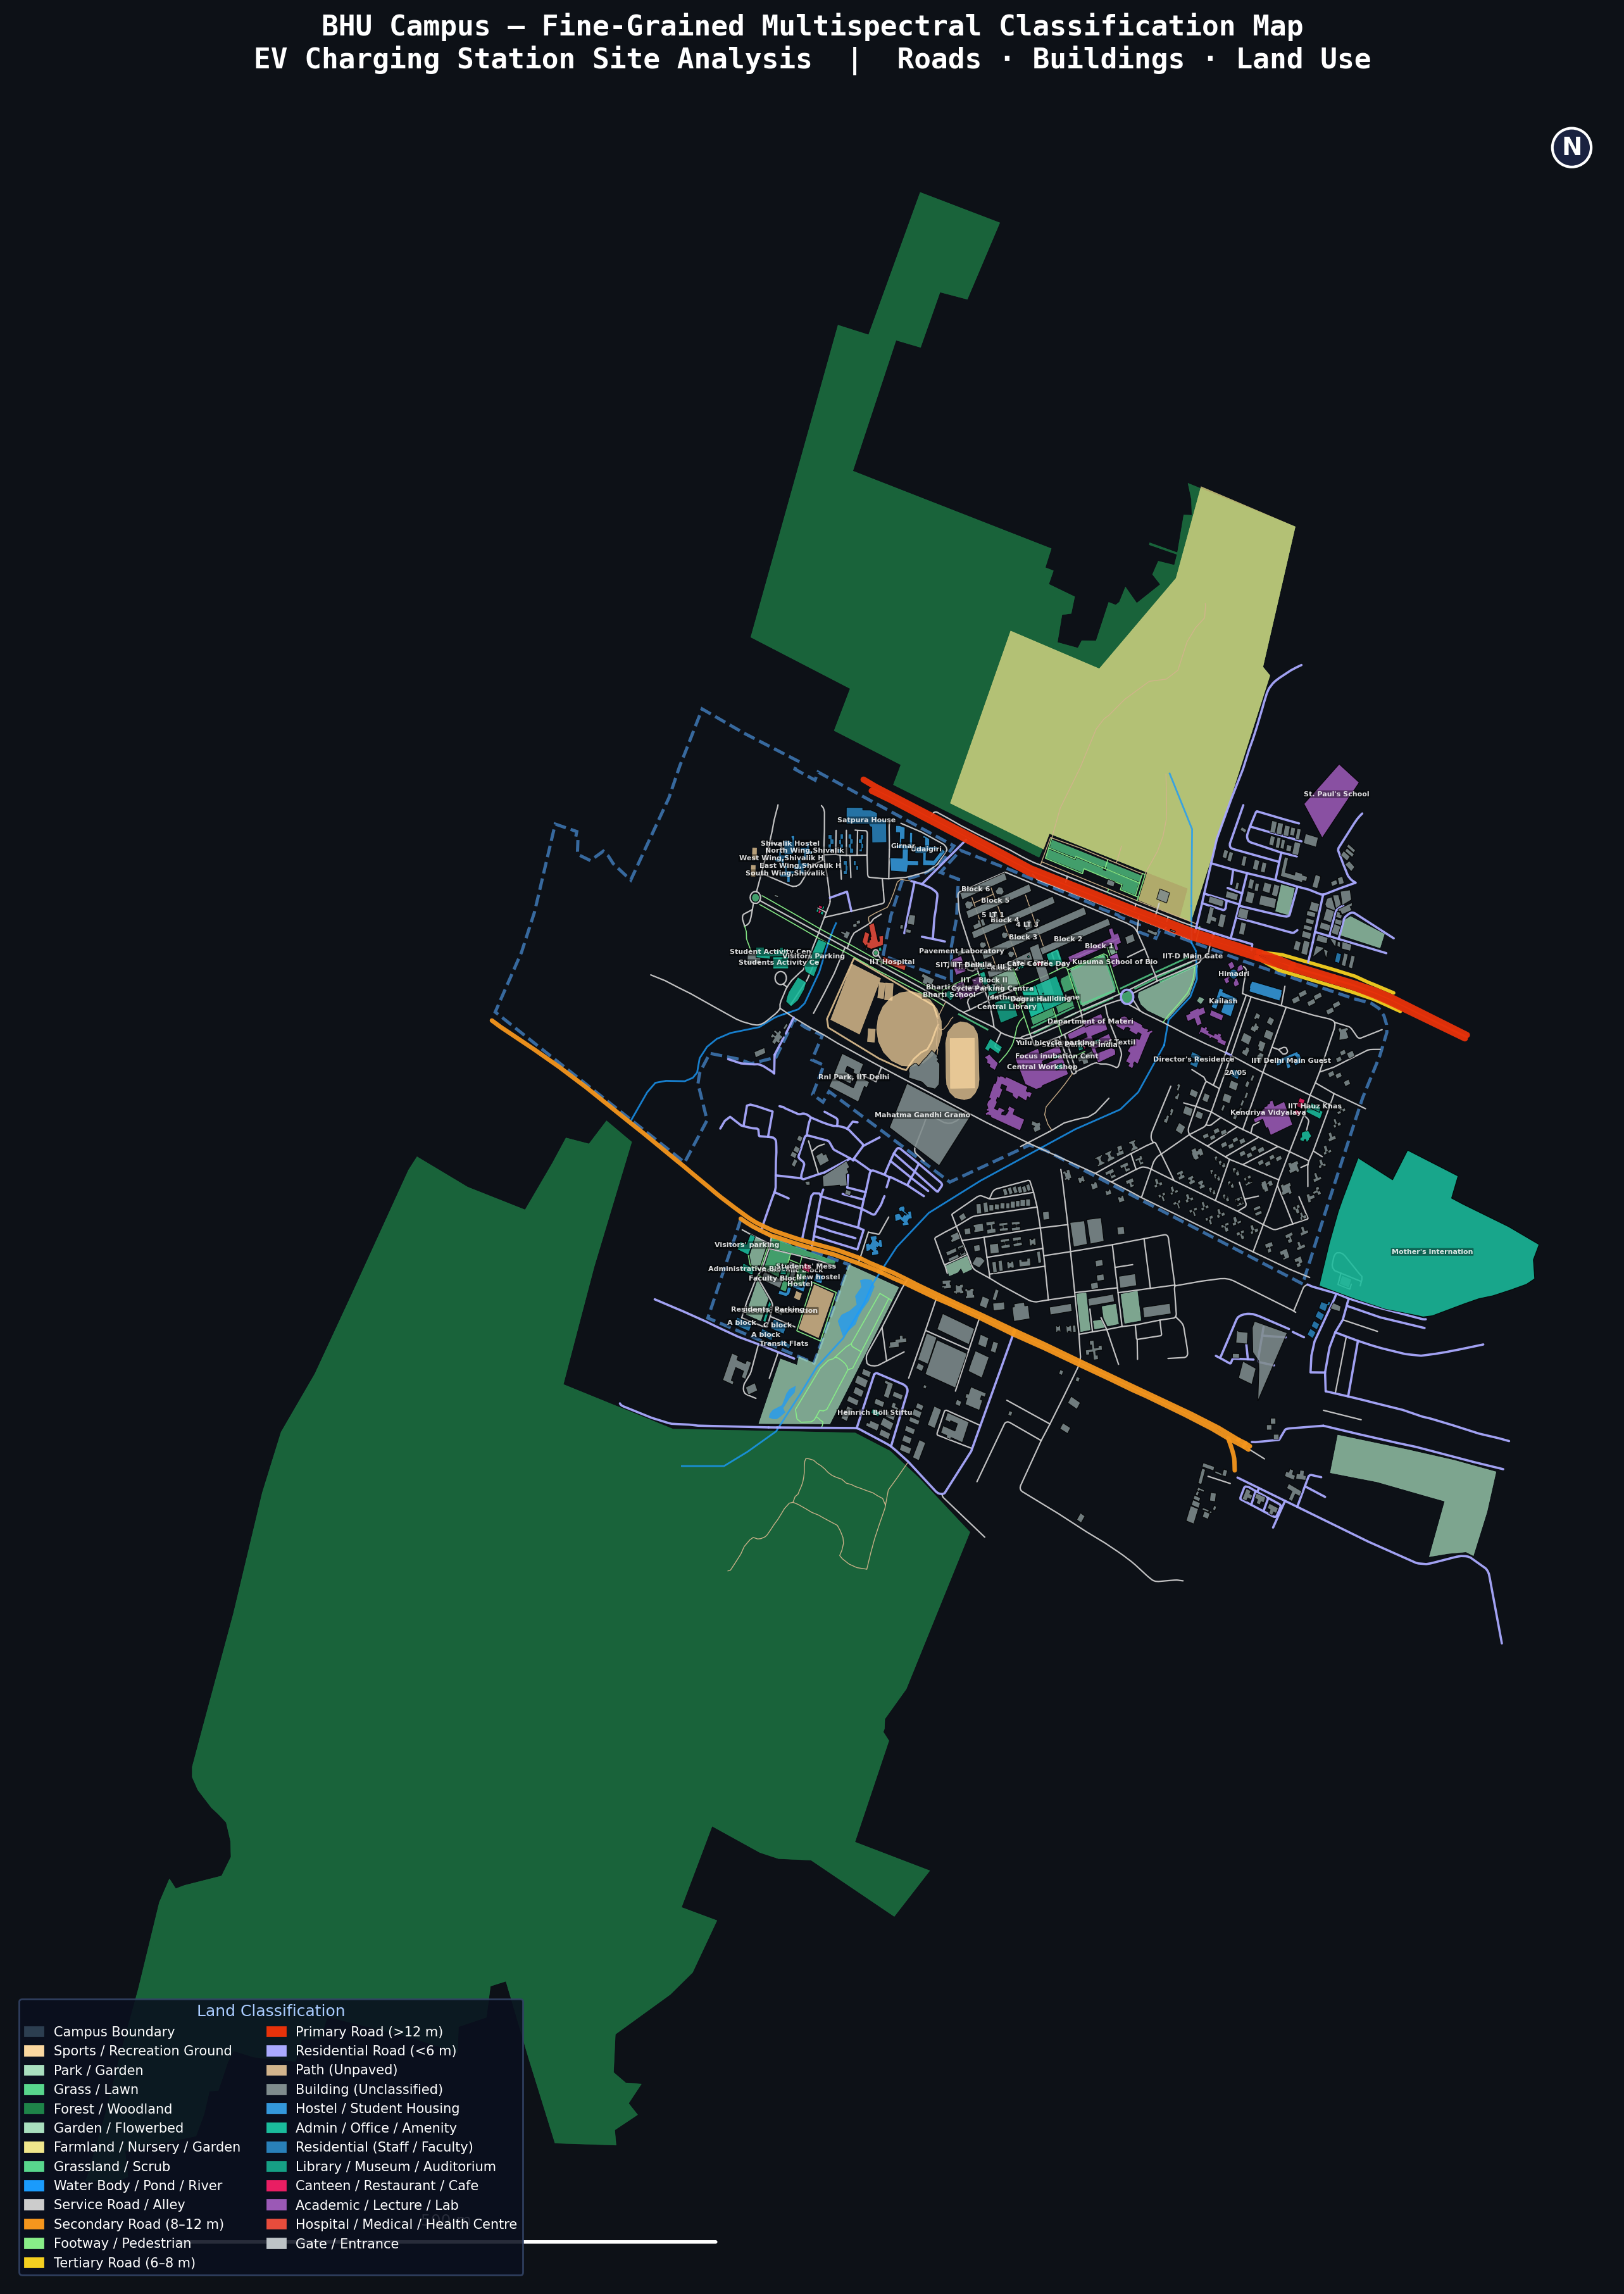
\includegraphics[width=\textwidth]{figures/iitd_multispectral.png}
    \caption{Multispectral Classification}
    \label{fig:iitd_multi}
\end{subfigure}
\hfill
\begin{subfigure}[b]{0.48\textwidth}
    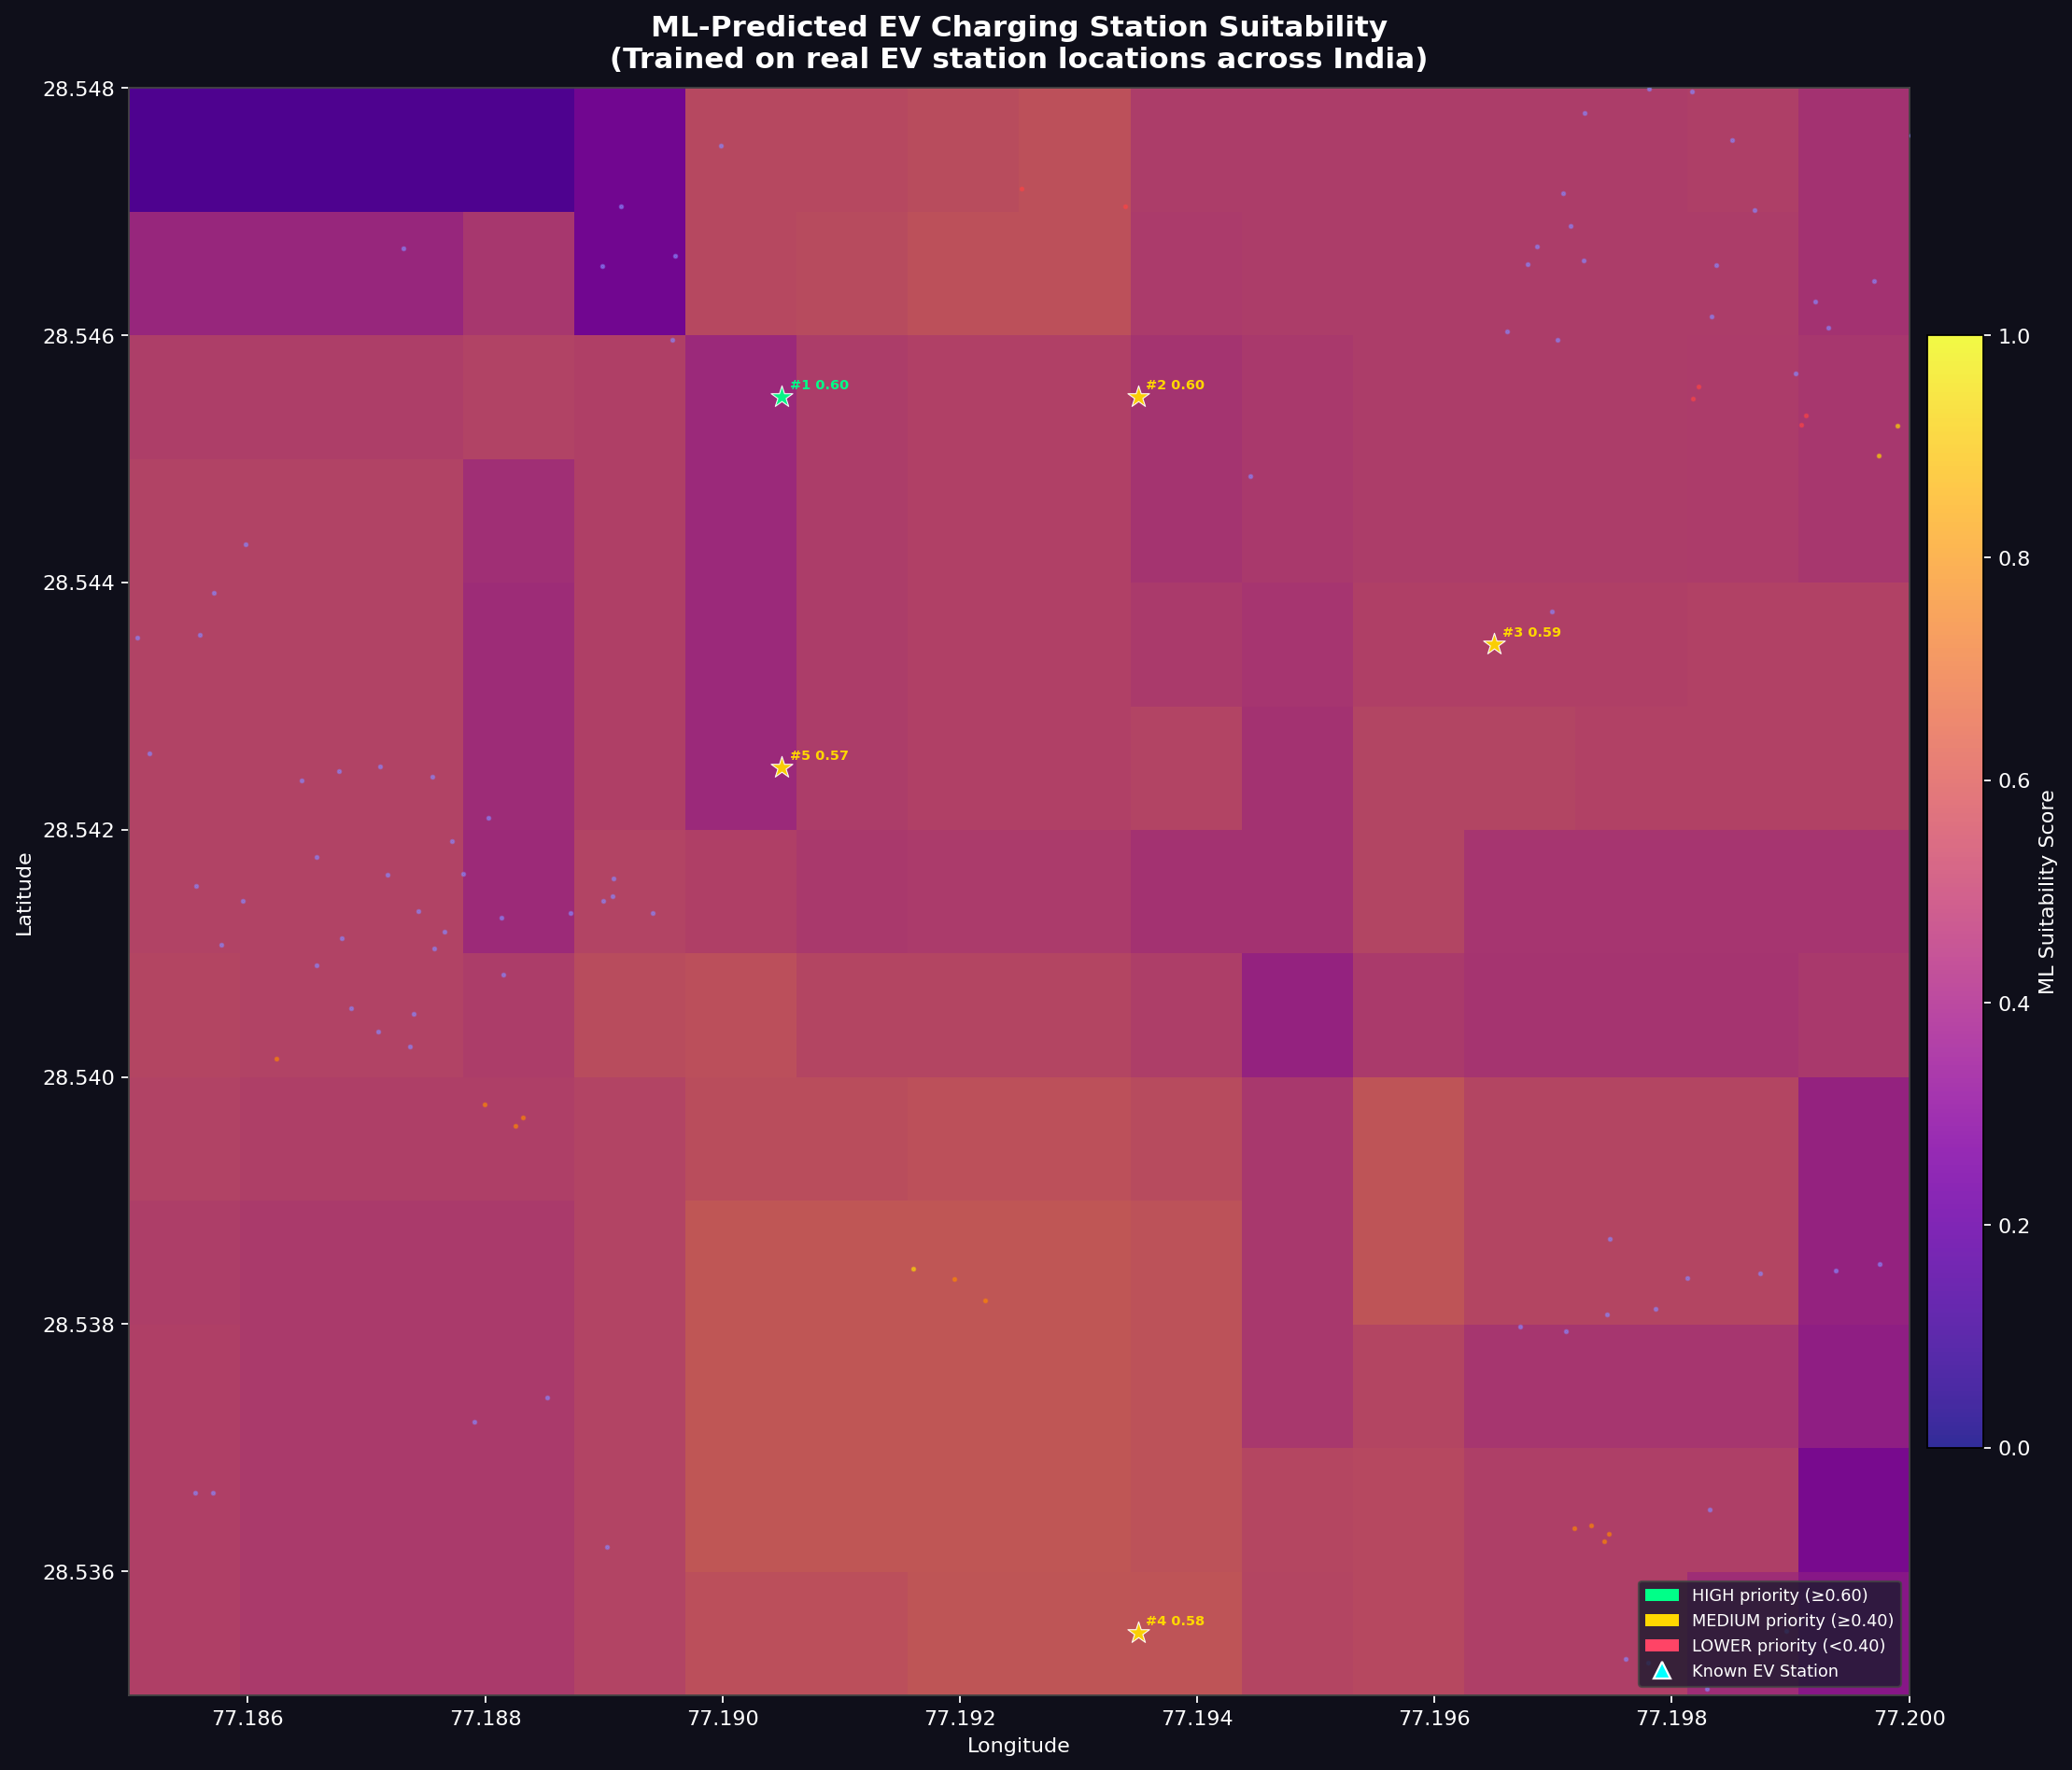
\includegraphics[width=\textwidth]{figures/iitd_ml_prediction.png}
    \caption{ML Prediction}
    \label{fig:iitd_ml}
\end{subfigure}
\caption{IIT Delhi — classification and ML prediction maps.}
\label{fig:iitd}
\end{figure}

\begin{table}[H]
\centering
\caption{IIT Delhi — ML-predicted top EV candidate zones.}
\label{tab:iitd_ml}
\begin{tabular}{@{}rccl@{}}
\toprule
\textbf{Rank} & \textbf{Latitude} & \textbf{Longitude} & \textbf{ML Score / Tier} \\
\midrule
1 & 28.5455 & 77.1905 & 0.6003 / HIGH \\
2 & 28.5455 & 77.1935 & 0.5982 / MEDIUM \\
3 & 28.5435 & 77.1965 & 0.5916 / MEDIUM \\
4 & 28.5355 & 77.1935 & 0.5770 / MEDIUM \\
5 & 28.5425 & 77.1905 & 0.5722 / MEDIUM \\
\bottomrule
\end{tabular}
\end{table}

\textbf{Observations:}
\begin{itemize}
    \item The model's top candidate (\#1, score 0.6003) is rated 
    HIGH priority — the only HIGH-priority result among the campus 
    case studies.
    \item This location corresponds to the northern area of the IIT 
    Delhi campus near the main gate and residential zones — a 
    sensible placement for real-world EV charger deployment.
    \item The model successfully generalised from the training data 
    (which included various Indian cities) to an entirely unseen 
    campus in a different state.
\end{itemize}

\subsection{Case Study 3: Majestic Area, Bangalore}

\begin{figure}[H]
\centering
\begin{subfigure}[b]{0.48\textwidth}
    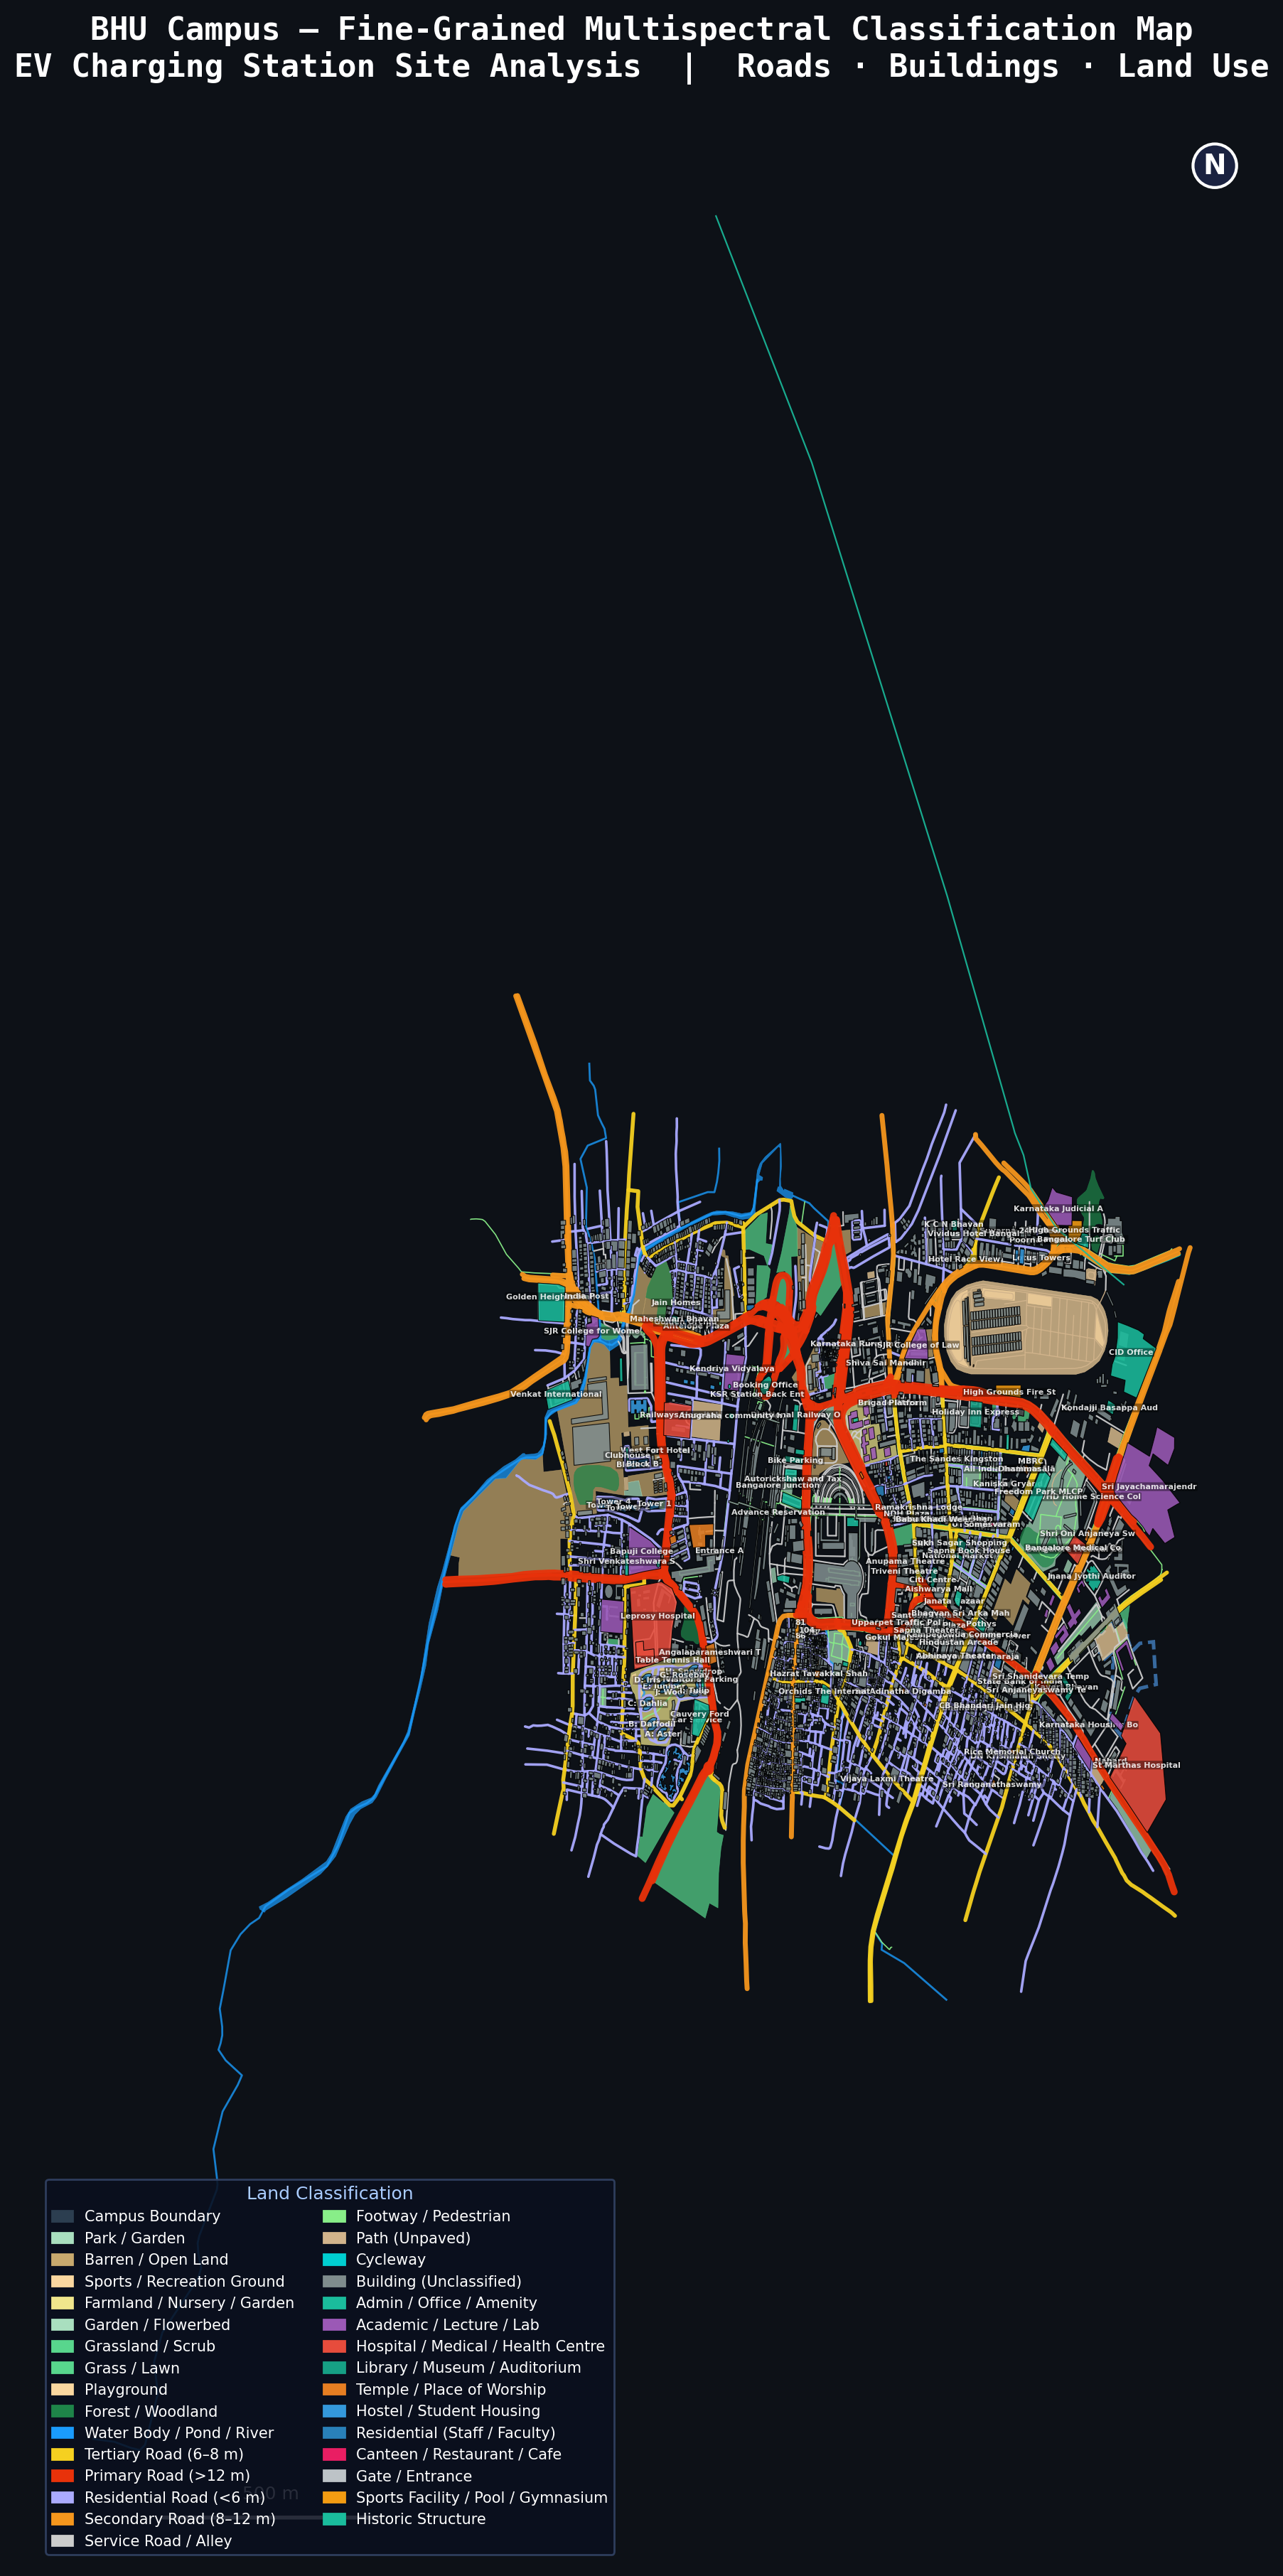
\includegraphics[width=\textwidth]{figures/majestic_multispectral.png}
    \caption{Multispectral Classification}
    \label{fig:maj_multi}
\end{subfigure}
\hfill
\begin{subfigure}[b]{0.48\textwidth}
    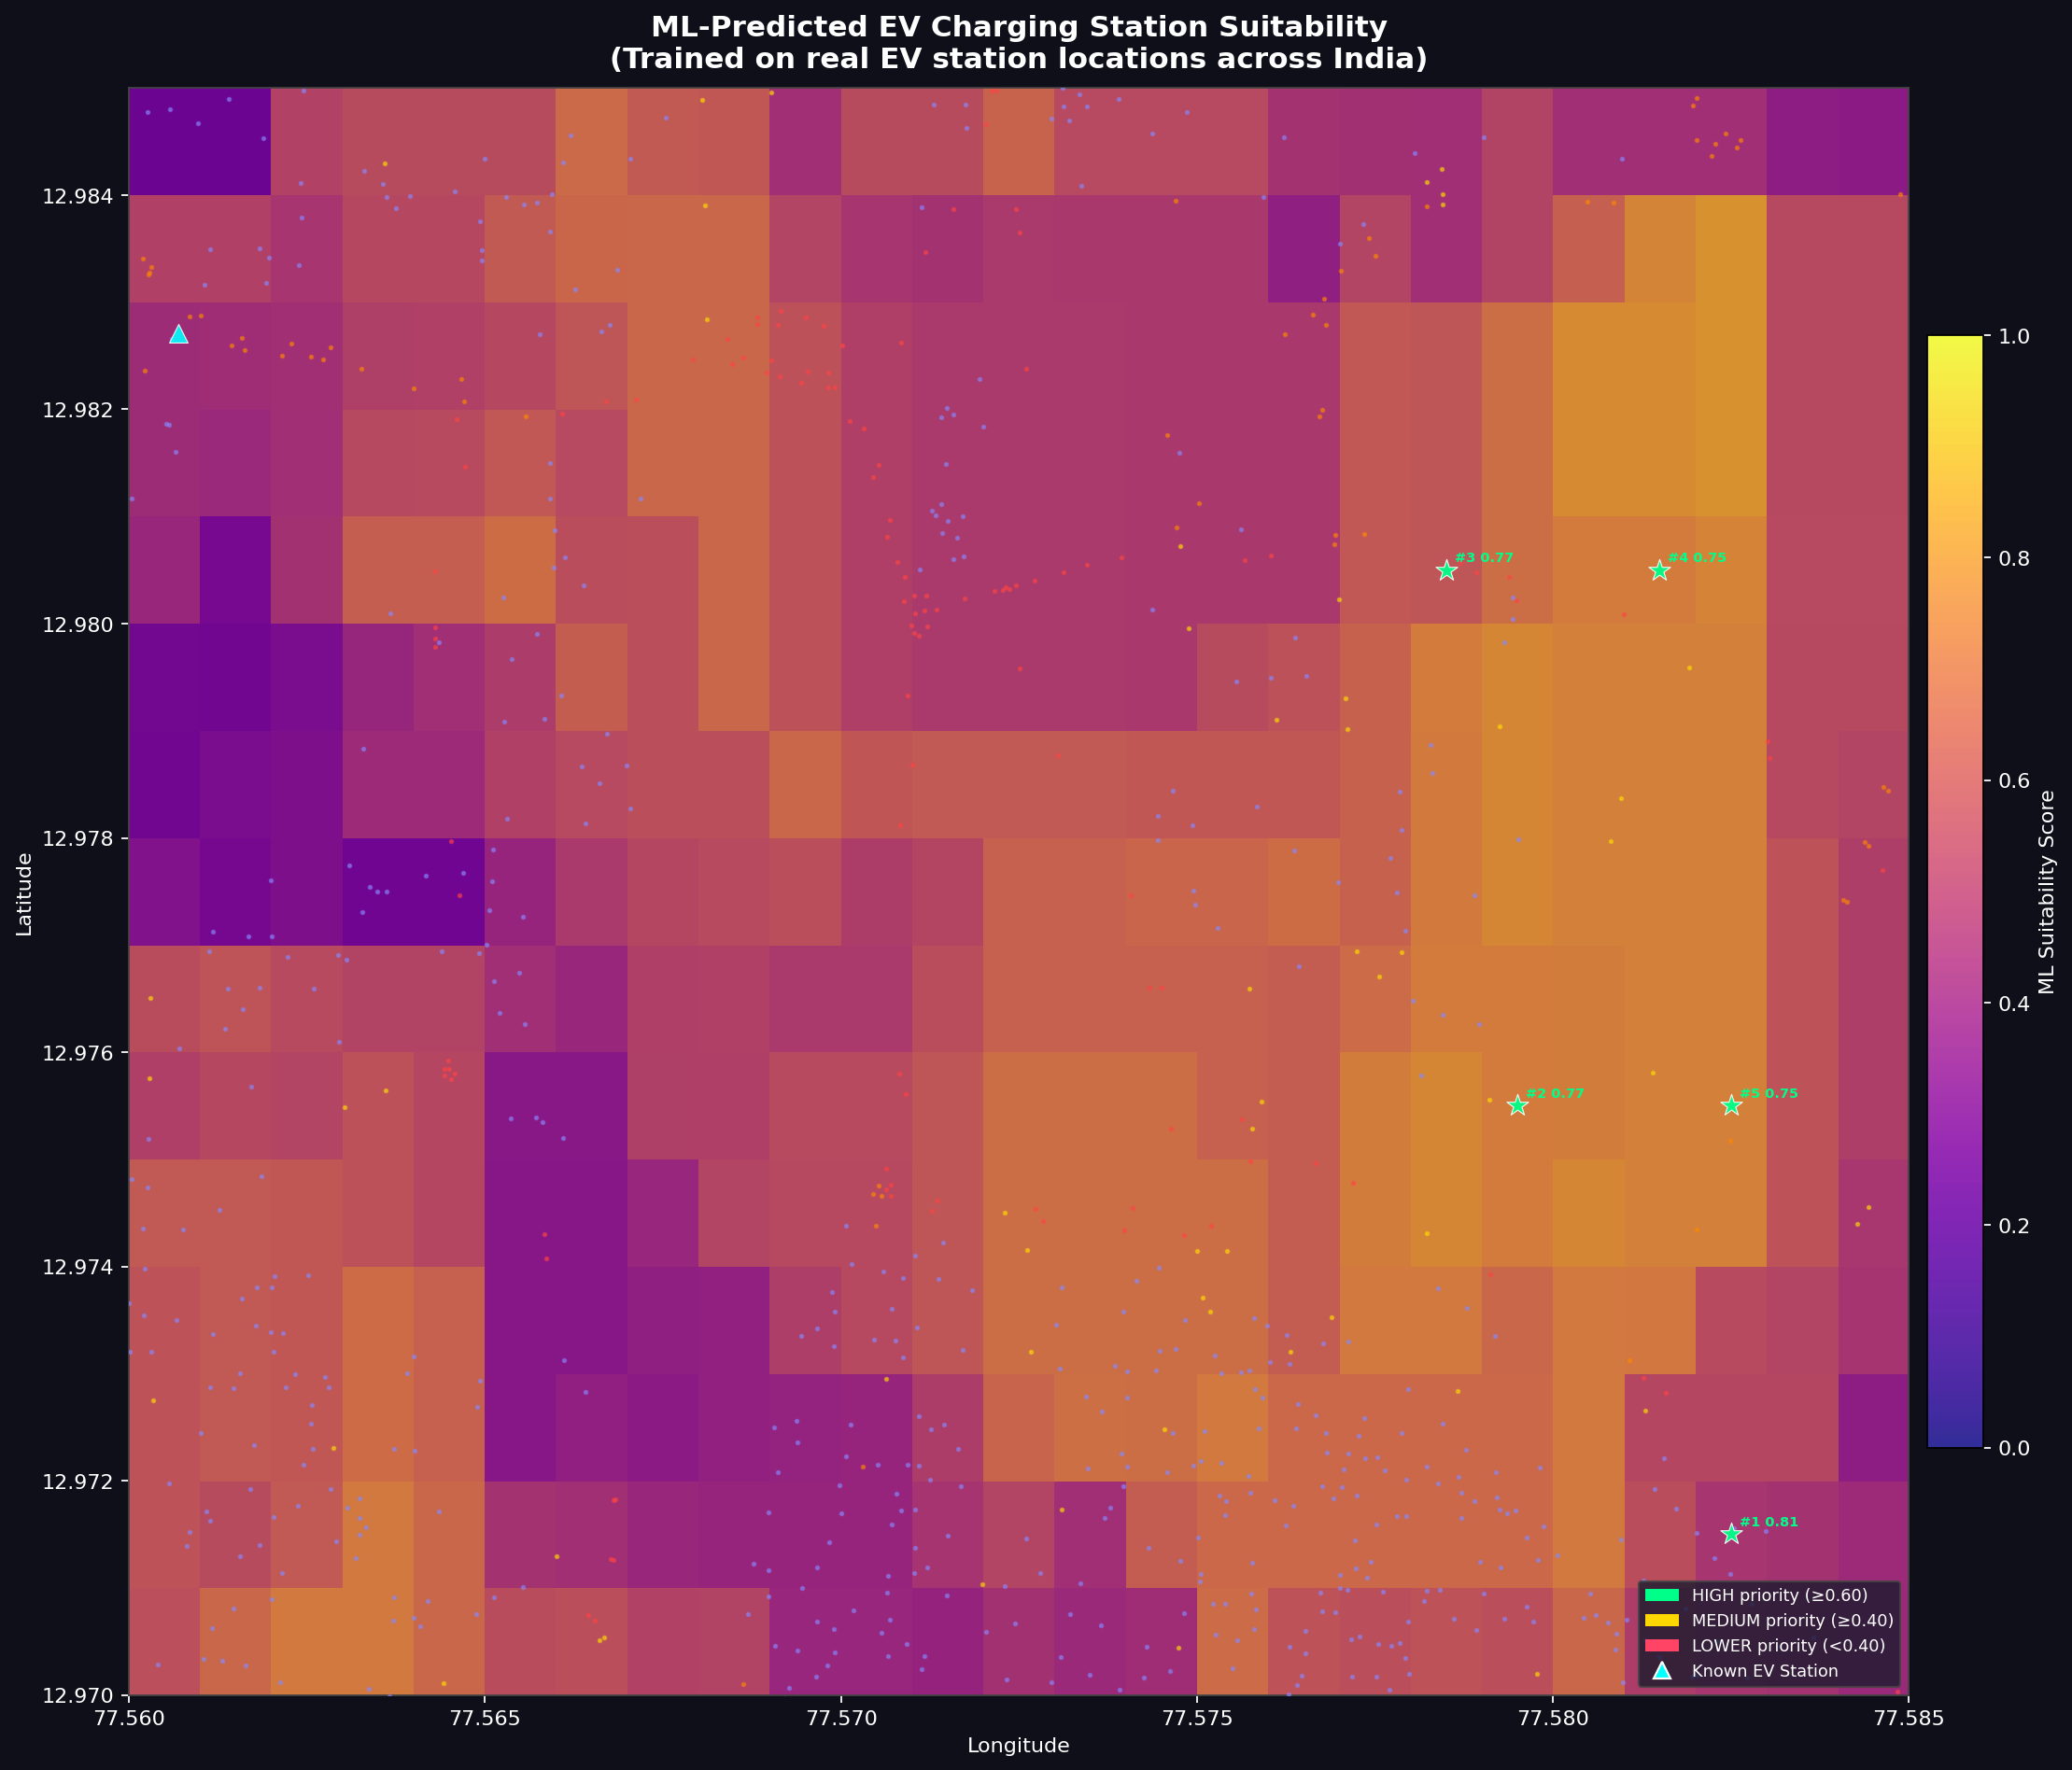
\includegraphics[width=\textwidth]{figures/majestic_ml_prediction.png}
    \caption{ML Prediction}
    \label{fig:maj_ml}
\end{subfigure}
\caption{Bangalore Majestic — classification and ML prediction maps.}
\label{fig:majestic}
\end{figure}

\begin{table}[H]
\centering
\caption{Bangalore Majestic — ML-predicted top EV candidate zones.}
\label{tab:majestic_ml}
\begin{tabular}{@{}rccl@{}}
\toprule
\textbf{Rank} & \textbf{Latitude} & \textbf{Longitude} & \textbf{ML Score / Tier} \\
\midrule
1 & 12.9715 & 77.5825 & 0.8111 / HIGH \\
2 & 12.9755 & 77.5795 & 0.7715 / HIGH \\
3 & 12.9805 & 77.5785 & 0.7715 / HIGH \\
4 & 12.9805 & 77.5815 & 0.7537 / HIGH \\
5 & 12.9755 & 77.5825 & 0.7510 / HIGH \\
\bottomrule
\end{tabular}
\end{table}

\textbf{Observations:}
\begin{itemize}
    \item \textbf{All five top candidates are rated HIGH priority}, 
    with scores ranging from 0.75 to 0.81 — significantly higher 
    than the campus case studies.
    \item This aligns with expectations: Majestic is a dense 
    commercial and transit hub with a major bus terminus, railway 
    station, metro station, and extensive commercial activity.
    \item The model correctly identifies the high-density urban 
    core as ideal for EV infrastructure — consistent with 
    Bangalore's actual EV charging deployment patterns.
    \item The OSM file for Majestic was 9.0~MB (compared to 3.4~MB 
    for BHU), reflecting much higher infrastructure density.
\end{itemize}

\subsection{Comparative Analysis}

\begin{table}[H]
\centering
\caption{Comparative summary across three test sites.}
\label{tab:comparison}
\begin{tabular}{@{}lccc@{}}
\toprule
\textbf{Metric} & \textbf{BHU Varanasi} & \textbf{IIT Delhi} & \textbf{Majestic, Bangalore} \\
\midrule
OSM file size & 3.4~MB & 1.9~MB & 9.0~MB \\
Area type & University campus & University campus & Urban commercial \\
Top ML score & 0.5856 & 0.6003 & 0.8111 \\
HIGH-tier candidates & 0 & 1 & 5 \\
MEDIUM-tier candidates & 7 & 4 & 0 \\
Key prediction zones & IIT core, library & Main gate, residences & Transit hub, commercial \\
\bottomrule
\end{tabular}
\end{table}

The comparative results demonstrate that:
\begin{enumerate}
    \item The model meaningfully differentiates between area types — 
    dense urban zones score much higher than semi-rural campuses.
    \item Within campuses, the model favours areas near main roads, 
    parking, and high-traffic amenities.
    \item The model generalises across geographies (Varanasi, Delhi, 
    Bangalore) without retraining.
\end{enumerate}


% ============================================================================
%                  7. CHALLENGES AND LIMITATIONS
% ============================================================================
\section{Challenges and Limitations}

\subsection{Technical Challenges Encountered}

\begin{enumerate}
    \item \textbf{Non-numeric CSV data:} The EV station CSV contained 
    latitude/longitude values stored as strings with embedded 
    whitespace, causing \texttt{TypeError} during geometric 
    calculations. Fixed by applying \texttt{pd.to\_numeric()} with 
    \texttt{errors='coerce'} and \texttt{dropna()}.
    
    \item \textbf{Unicode encoding on Windows:} Progress indicators 
    using UTF-8 checkmarks (\checkmark) caused 
    \texttt{UnicodeEncodeError} on Windows terminals using cp1252 
    encoding. Resolved by replacing Unicode symbols with ASCII 
    equivalents.
    
    \item \textbf{Overpass API rate limiting:} The free Overpass API 
    imposes rate limits. Mitigated by adding 2-second delays between 
    requests, implementing exponential backoff retries, and caching 
    training data to disk.
    
    \item \textbf{OSM data quality:} Many buildings in the BHU 
    dataset are tagged only as \texttt{building=yes} with no 
    functional information. This required extensive name-based keyword 
    matching as a fallback.
\end{enumerate}

\subsection{Limitations}

\begin{itemize}
    \item \textbf{No satellite/remote sensing data:} Classification 
    is purely from OSM vector tags, not actual multispectral imagery.
    
    \item \textbf{No electrical grid data:} The model does not 
    consider transformer capacity, substation proximity, or power 
    grid constraints.
    
    \item \textbf{No traffic data:} Real traffic volume counts are 
    not available from OSM. Road hierarchy serves as a proxy.
    
    \item \textbf{Model AUC = 0.678:} While above random chance, the 
    model's discriminative power is moderate. This is likely due to 
    feature limitations in OSM data and the noisy nature of the 
    negative sample generation.
    
    \item \textbf{No multipolygon support:} OSM relations 
    (multipolygon buildings, complex boundaries) are not parsed; only 
    simple way polygons are processed.
    
    \item \textbf{Height data sparse:} Most buildings lack explicit 
    \texttt{height=*} tags in OSM, so 3D heights are category 
    defaults.
\end{itemize}


% ============================================================================
%                      8. FUTURE WORK
% ============================================================================
\section{Future Work}

\begin{enumerate}
    \item \textbf{Enriched training data:} Incorporate global EV 
    station datasets (OpenChargeMap API with 250,000+ locations 
    worldwide) to improve model AUC.
    
    \item \textbf{Feature augmentation:} Add population density 
    (census data), traffic flow estimates (Google Roads API), 
    electrical grid proximity (power infrastructure OSM tags), and 
    elevation data.
    
    \item \textbf{Advanced models:} Experiment with XGBoost, 
    LightGBM, and spatial graph neural networks (GNNs) for improved 
    spatial reasoning.
    
    \item \textbf{Interactive web dashboard:} Build a Folium/Leaflet 
    web map with interactive layers, filtering, and real-time Overpass 
    queries.
    
    \item \textbf{Real-time demand modelling:} Integrate EV 
    registration data and ride-hailing patterns to model time-varying 
    charging demand.
    
    \item \textbf{Multi-objective optimisation:} Formulate station 
    placement as a facility location problem minimising total travel 
    distance while maximising coverage equity.
    
    \item \textbf{Satellite image fusion:} Combine OSM features with 
    actual multispectral satellite imagery (Sentinel-2) for true 
    remote-sensing-based analysis.
\end{enumerate}


% ============================================================================
%                      9. CONCLUSION
% ============================================================================
\section{Conclusion}

This project demonstrates an end-to-end, \textbf{open-data-driven} 
approach to identifying optimal Electric Vehicle charging station 
locations. By combining:

\begin{itemize}
    \item A \textbf{multispectral classification engine} that 
    translates raw OSM tags into rich, colour-coded spatial maps,
    \item A \textbf{heuristic scoring model} that ranks zones based 
    on domain knowledge of EV infrastructure requirements,
    \item A \textbf{supervised Random Forest classifier} trained on 
    real EV station coordinates from across India,
\end{itemize}

\noindent the system provides actionable, spatially-explicit 
recommendations for EV charger deployment on any geographic area 
available in OpenStreetMap — without requiring proprietary software, 
GIS licenses, or satellite imagery.

The pipeline was validated on three diverse sites: a large university 
campus (BHU), a compact technical institute (IIT Delhi), and a dense 
urban commercial zone (Bangalore Majestic). Results demonstrate:

\begin{enumerate}
    \item The model correctly identifies high-traffic urban zones 
    (Majestic: all 5 candidates rated HIGH, scores 0.75--0.81) while 
    assigning moderate scores to less urbanised campuses.
    \item Feature importance analysis reveals that POI density, 
    amenity count, and restaurant/cafe presence are the strongest 
    predictors — aligning with real-world station placement logic.
    \item The system generalises across Indian cities without 
    retraining.
\end{enumerate}

The entire codebase is open-source, lightweight ($\sim$1,800 lines 
of Python), and runs on any machine with Python 3.8+ and standard 
ML libraries — no GPU required.


% ============================================================================
%                      10. HOW TO RUN
% ============================================================================
\section{Reproducibility and Usage}

\subsection{Installation}

\begin{lstlisting}[language=bash, caption={Setting up the environment.}]
# Create and activate virtual environment
python -m venv myenv
myenv\Scripts\activate        # Windows
source myenv/bin/activate     # Linux/Mac

# Install dependencies
pip install -r requirements.txt
\end{lstlisting}

\subsection{Running the Pipeline}

\begin{lstlisting}[language=bash, caption={Running the analysis.}]
# Full pipeline (classification + ML prediction)
python main.py --osm map.osm --output ./output

# Training mode (one-time, needs internet)
python main.py --train --csv ev-charging-stations-india.csv

# Prediction on a new map (offline)
python main.py --osm new_area.osm --output ./output_new
\end{lstlisting}

\subsection{Obtaining OSM Data}

Any area in the world can be analysed by downloading its OSM data:

\begin{lstlisting}[language=bash, caption={Downloading OSM data via Overpass API.}]
# Example: IIT Delhi bounding box
# URL: https://overpass-api.de/api/map?bbox=77.185,28.535,77.200,28.548

# Or use openstreetmap.org > Export > select area > Export
\end{lstlisting}


% ============================================================================
%                      REFERENCES
% ============================================================================
\newpage
\begin{thebibliography}{9}

\bibitem{niti2022}
NITI Aayog, Government of India, ``Electric Vehicle Charging 
Infrastructure — Handbook for Urban Planners,'' 2022.

\bibitem{osm}
OpenStreetMap Contributors, ``OpenStreetMap,'' Available: 
\url{https://www.openstreetmap.org}. [Accessed: April 2026].

\bibitem{overpass}
Overpass API, ``Overpass API — Query Language for OpenStreetMap,'' 
Available: \url{https://wiki.openstreetmap.org/wiki/Overpass_API}. 
[Accessed: March 2026].

\bibitem{sklearn}
F. Pedregosa \textit{et al.}, ``Scikit-learn: Machine Learning in 
Python,'' \textit{Journal of Machine Learning Research}, vol. 12, 
pp. 2825--2830, 2011.

\bibitem{breiman2001}
L. Breiman, ``Random Forests,'' \textit{Machine Learning}, vol. 45, 
no. 1, pp. 5--32, 2001.

\bibitem{fame2}
Ministry of Heavy Industries, Government of India, ``FAME India 
Scheme Phase II,'' 2019. Available: 
\url{https://fame2.heavyindustries.gov.in/}.

\bibitem{frlm}
M.~Kuby and S.~Lim, ``The Flow-Refueling Location Model for 
Alternative-Fuel Vehicles,'' \textit{Socio-Economic Planning 
Sciences}, vol. 39, no. 2, pp. 125--145, 2005.

\bibitem{matplotlib}
J.~D.~Hunter, ``Matplotlib: A 2D Graphics Environment,'' 
\textit{Computing in Science \& Engineering}, vol. 9, no. 3, 
pp. 90--95, 2007.

\end{thebibliography}

\end{document}
